\documentclass[10pt,a4paper,twocolumn]{article}
\usepackage[a4paper,margin=2.0cm,columnsep=0.7cm]{geometry}
\usepackage[T1]{fontenc}
\usepackage{lmodern}
\usepackage{amsmath,amssymb}
\usepackage{graphicx}
\usepackage{booktabs}
\usepackage{float}
\usepackage{fancyhdr}
\usepackage{caption}
\usepackage{enumitem}
\usepackage[hidelinks]{hyperref}
\captionsetup{font=small,labelfont=bf}
\setlist{itemsep=1pt,topsep=3pt,leftmargin=*}
\graphicspath{{figures/}{../figures/}}
\setlength{\headheight}{14pt}
\pagestyle{fancy}
\fancyhf{}
\lhead{Computer Vision ( CS6350 )}
\rhead{Compute change in pose (3D) of a small object}
\cfoot{\thepage}
\renewcommand{\headrulewidth}{0.4pt}
\newcommand{\R}{\mathbf{R}}
\newcommand{\tv}{\mathbf{t}}
\newcommand{\K}{\mathbf{K}}
\newcommand{\X}{\mathbf{X}}
\newcommand{\x}{\mathbf{x}}
\newcommand{\n}{\mathbf{n}}
\sloppy

\begin{document}

% ------------------------------------------------------------------ title page
\onecolumn
\thispagestyle{empty}
\begin{center}
\vspace*{1.2cm}

\includegraphics[width=3.2cm]{iitm_logo.png}\\[1.2cm]
{\Large\scshape Indian Institute of Technology Madras}\\[2.2cm]
{\LARGE\bfseries (TPA 12)}\\[6pt]
{\LARGE\bfseries Compute change in pose (3D) of small objects}\\[1.4cm]
{\large\bfseries Course: CS6350}\\[0.5cm]
{\large Professor: Dr.\ Sukhendu Das}\\[1.6cm]
{\normalsize Members:}\\[0.4cm]
{\normalsize Sai Svanik Chiramana (ME23B195)}\\[2pt]
{\normalsize Sathwik Chanduluri (ME23B238)}
\end{center}
\newpage
\twocolumn[
\begin{@twocolumnfalse}
\begin{center}\textbf{Abstract}\end{center}
\begin{quote}
\small This work addresses the estimation of the change in three-dimensional pose of a small object from two RGB images when nothing else is known: neither the camera intrinsics, nor the location of the object, nor its category. The proposed pipeline first estimates the focal length from a dense point map predicted by MASt3R, then locates the object by segmenting the image with SAM~2.1 and identifying the segment whose motion is inconsistent with that of the background. Correspondences on the object are obtained with MASt3R, a homography and an essential matrix are fitted with MAGSAC++, the appropriate model is selected by the GRIC criterion, and the pose is recovered through a decomposition that resolves the two-fold ambiguity of planar scenes, followed by Levenberg--Marquardt refinement. The output comprises the relative rotation, the direction of translation and the root-mean-square reprojection error. On 56 held-out image pairs from four public datasets (TUM RGB-D, Objectron, CO3D and MVImgNet) covering twelve objects and scenes and viewpoint changes from under $1^\circ$ to $90^\circ$, the pipeline attains a median rotation error of $0.97^\circ$, a median translation-direction error of $1.79^\circ$ and a median reprojection error of 0.46\,px, within one point of AUC@$10^\circ$ of the same estimator supplied with the true camera and object mask. On a sequence of 38 frame pairs the per-axis mean absolute rotation errors are $0.43^\circ$, $0.34^\circ$ and $0.19^\circ$ for roll, pitch and yaw.

\smallskip\noindent\textit{Use of AI tools:} ChatGPT and Gemini were used to identify relevant reference papers, and Claude Code was used to assist in resolving errors in the code.
\end{quote}
\vspace{0.4cm}
\end{@twocolumnfalse}
]

% ------------------------------------------------------------------ 1
\section{Introduction}

\textbf{Estimating the six-degree-of-freedom pose change of an object from two images} is a basic problem in robotics, augmented reality and object tracking. The task considered here, TPA-12, asks for the relative rotation $\R$ and translation $\tv$ of a small object---a coin, key, mobile phone, purse, clock, plate or checkerboard---between two successive views taken from arbitrary viewpoints, together with reprojection error metrics that indicate the accuracy of the estimate. The objects may be nearly planar.

Three properties make the problem difficult. First, a small object occupies a small fraction of the image, so it yields few correspondences while the background yields many; correspondences on the background describe the motion of the background, not of the object. Second, small objects are frequently weakly textured or specular, which defeats keypoint detectors. Third, near-planar objects make the essential matrix ill-conditioned and admit two physically valid poses. In addition, two views determine the translation only up to scale, so its direction is estimated and its magnitude requires an external reference such as the object's size.

In the setting addressed in this report, \emph{only the two images are available}. The camera intrinsics must therefore be estimated, and the object must be found without a bounding box, mask or class name. The contributions are:
\begin{itemize}
  \item a fully automatic pipeline that estimates the focal length, identifies the moved object by geometric and photometric consistency tests, and computes the pose with a planar/non-planar model choice;
  \item a resolution of the planar two-fold ambiguity that is applied even when the essential matrix is selected;
  \item an evaluation on four real-image datasets with tuning and test splits, viewpoint changes up to $90^\circ$, and a comparison with the same estimator given the true camera and mask.
\end{itemize}

% ------------------------------------------------------------------ 2
\section{Methodology}

\subsection*{Pipeline Overview}
The processing chain is shown in Figure~\ref{fig:pipeline}. The front end supplies the two quantities that are not given---the intrinsic matrix and the object region---and the remainder computes the pose from correspondences on the object:
\begin{center}\small
Focal length $\rightarrow$ Object region $\rightarrow$ ROI extraction $\rightarrow$ Matching $\rightarrow$ $H$/$E$ estimation $\rightarrow$ Model selection $\rightarrow$ Decomposition $\rightarrow$ Refinement $\rightarrow$ Output.
\end{center}

\begin{figure*}[t]
  \centering
  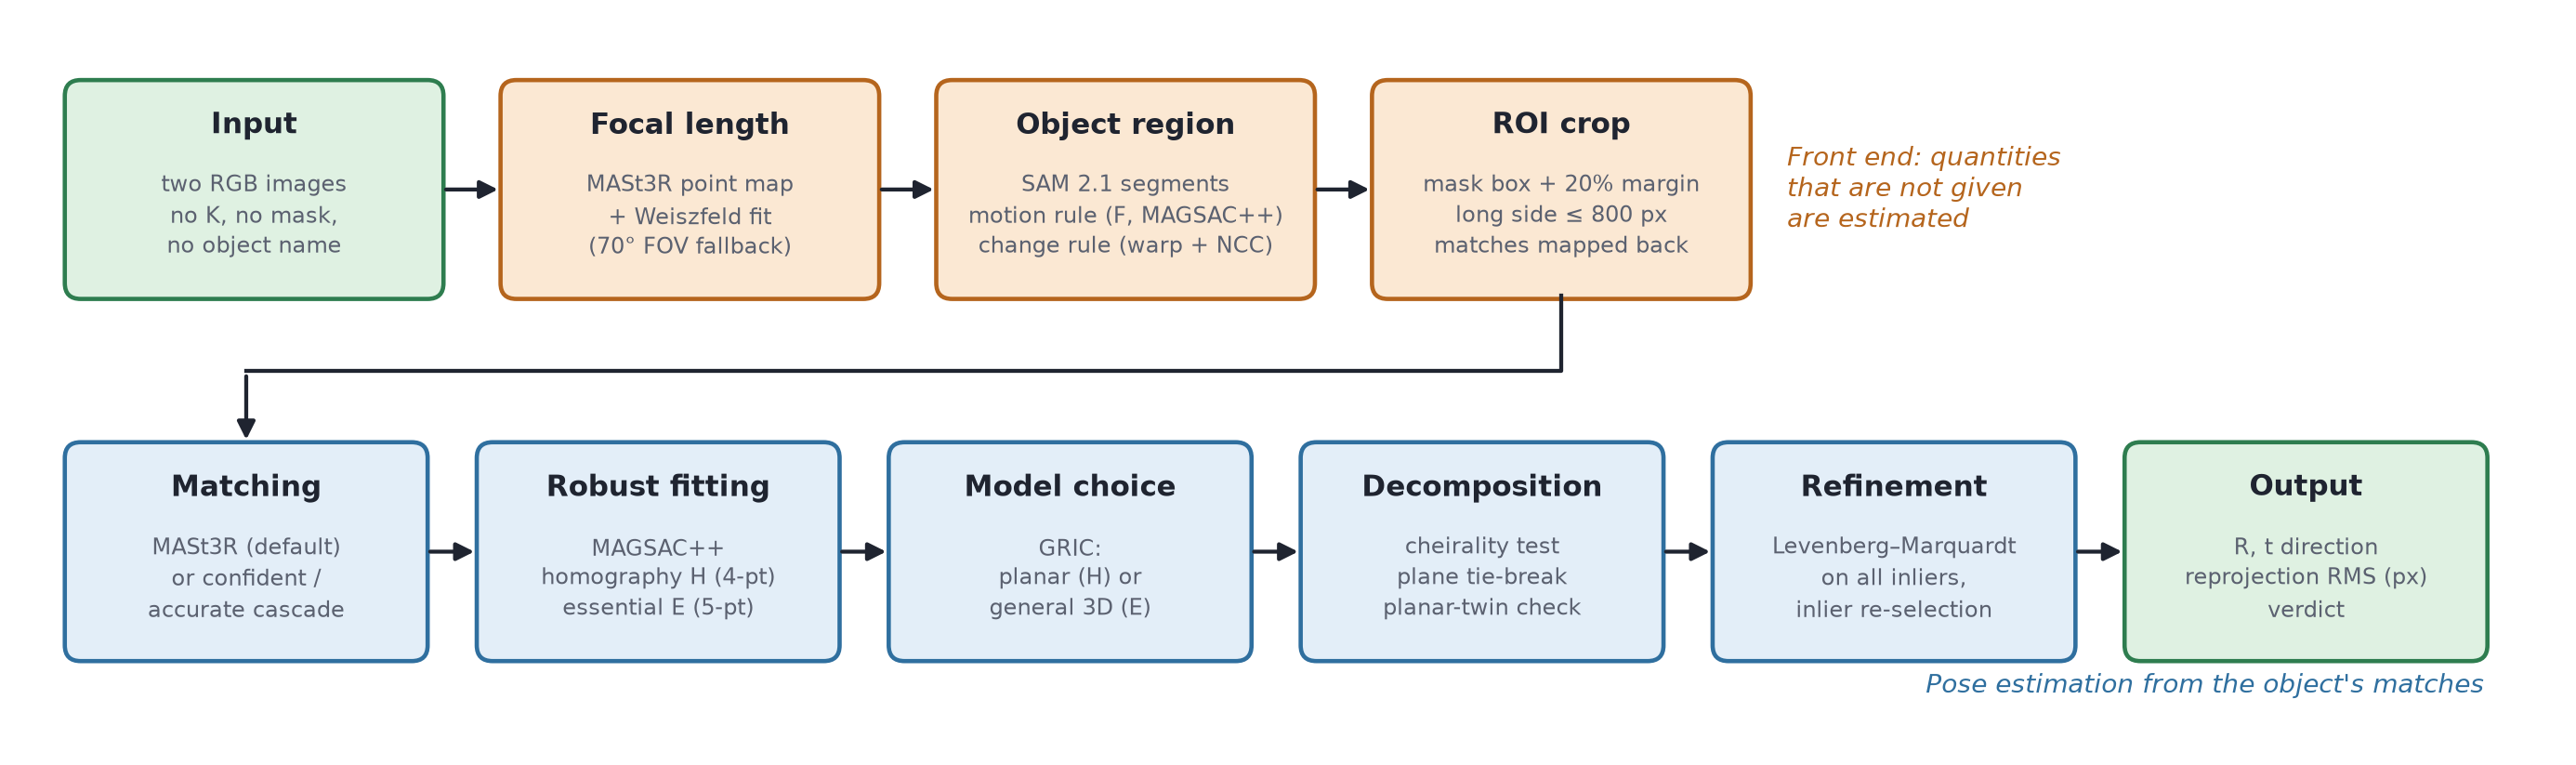
\includegraphics[width=\textwidth]{pipeline.png}
  \caption{The two-image pipeline. The front end (orange) estimates the focal length and the object region; the pose is computed from correspondences on the object (blue). Only the two RGB images are used.}
  \label{fig:pipeline}
\end{figure*}

\subsection*{Dataset and Experimental Setup}
Four public datasets with ground-truth camera poses are used (Figure~\ref{fig:datasets}). TUM RGB-D~\cite{tum} provides indoor video with motion-capture poses; the RGB images alone are used, with poses interpolated (linear for position, spherical linear for orientation) to the image timestamps. Objectron~\cite{objectron} provides phone videos of objects with AR-tracked poses; only the selected frames are decoded. CO3D~\cite{co3d} and MVImgNet~\cite{mvimgnet} provide object-centric image sequences with structure-from-motion poses, converted to the OpenCV convention. Twelve objects or scenes are used: two poster scenes, two three-dimensional structures and a checkerboard (TUM); book, laptop and cereal box (Objectron); mobile phone and handbag (CO3D); key and watch (MVImgNet). Seven are near-planar and five are three-dimensional.

For a pair of frames with world-to-camera poses $(\R_1,\tv_1)$ and $(\R_2,\tv_2)$, the ground-truth relative pose is
\begin{equation}
  \R_{gt} = \R_2\R_1^\top, \qquad \tv_{gt} = \tv_2 - \R_{gt}\tv_1 ,
\end{equation}
which maps a point from the first camera's frame to the second's, $\X_2 = \R\X_1 + \tv$. Every threshold in the pipeline was set on tuning sequences (sequences 01--03 of each object and the first 30\% of each TUM video); all results are on the remaining test sequences. The test set comprises 56 pairs in three groups: 32 pairs with one pair per object and viewpoint bin (5--15$^\circ$, 15--30$^\circ$, 30--60$^\circ$), 10 consecutive-frame TUM pairs (rotation below $1^\circ$), and 14 pairs with 60--90$^\circ$ of viewpoint change.

\begin{figure*}[t]
  \centering
  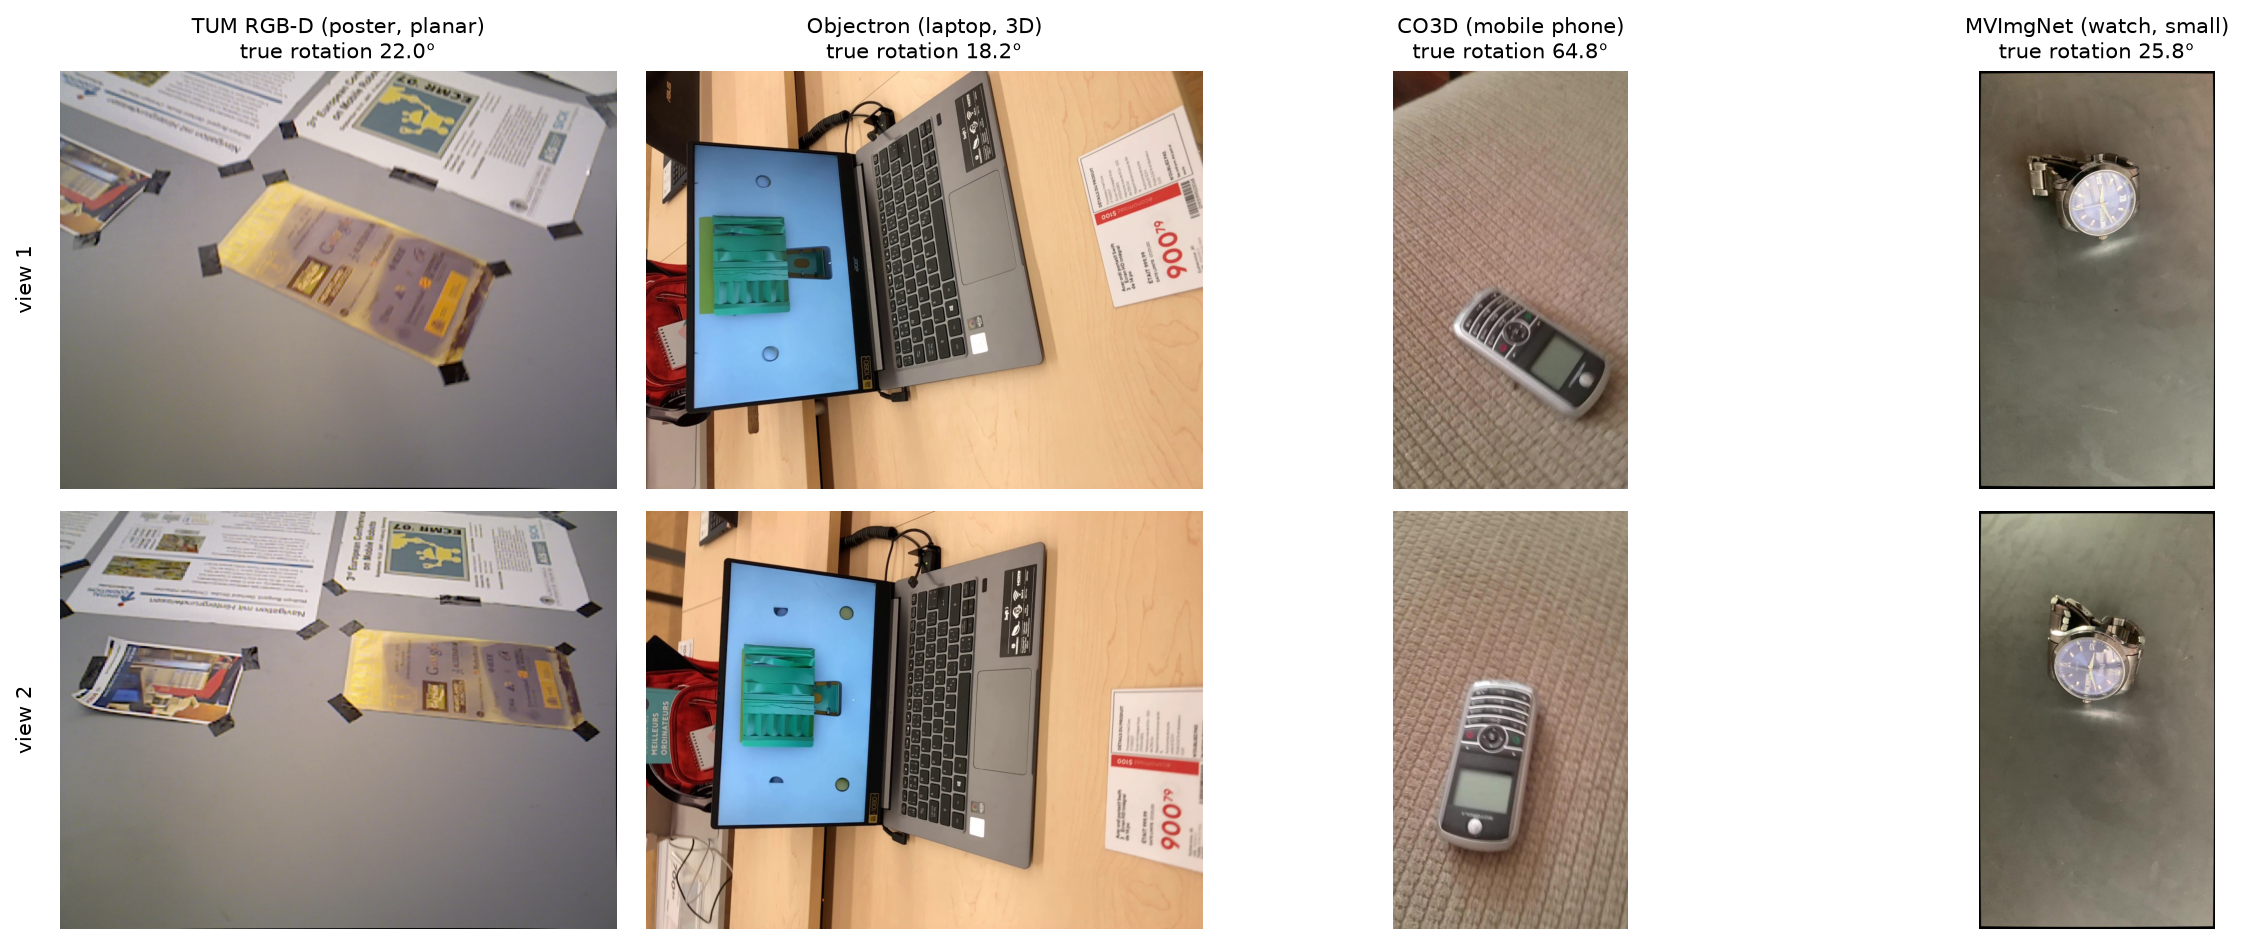
\includegraphics[width=0.92\textwidth]{datasets.png}
  \caption{One test pair from each dataset with its ground-truth rotation angle.}
  \label{fig:datasets}
\end{figure*}

\subsection*{Dataset Preprocessing}
All four datasets are converted offline into a common form: image frames, a pixel intrinsic matrix $\K$, a world-to-camera pose $(\R_i,\tv_i)$ in the OpenCV convention ($x$ right, $y$ down, $z$ forward) and, where available, an object mask (Figure~\ref{fig:dataprep}). This step prepares the evaluation data and its ground truth only; the pipeline itself receives just the two images.

\textbf{TUM RGB-D.} Five fr3 sequences are used, with the RGB images only. Motion capture provides camera-to-world poses at about 100\,Hz while the RGB camera runs at about 30\,Hz, so the pose of each frame is interpolated at its timestamp---linearly for the position and by spherical linear interpolation for the orientation---and then inverted to world-to-camera. The camera axes already follow the OpenCV convention, and in these scenes the textured scene itself is the region of interest.

\textbf{Objectron.} Each sequence is a phone video with an annotation file that gives, for every frame, the ARKit camera pose, the intrinsics and the 3D bounding box of the object. The annotation is parsed first and the pairs are selected from the poses; the video is then decoded once and only the frames belonging to selected pairs are stored (JPEG, quality 95). Frames are rotated from portrait to landscape to match the intrinsics, the ARKit axes ($y$ up, $z$ backward) are converted with $F=\mathrm{diag}(1,-1,-1)$, and the object mask is the filled convex hull of the projected box corners.

\textbf{CO3D.} A full category occupies 90--140\,GB, so only the required files are read from the remote archives with HTTP range requests: the ten sequences per category with the highest viewpoint-quality score, and from each only the images, masks and cameras. The PyTorch3D cameras (row-vector convention, $x$ left, $y$ up, intrinsics in normalised device coordinates) are converted to OpenCV by
\begin{gather}
  \R_{cv} = F\,\R^\top,\quad \tv_{cv} = F\,\tv,\quad F=\mathrm{diag}(-1,-1,1),\\
  f_{px} = f_{ndc}\,s,\qquad s=\min(W,H)/2,\\
  \mathbf{c}_{px} = (W/2,\,H/2) - \mathbf{p}_{ndc}\,s ,
\end{gather}
and the dataset masks are used as object regions.

\textbf{MVImgNet.} Each sequence contains about 30 phone frames, a background-removed cut-out per frame whose alpha channel provides the object mask, and a COLMAP model with one radial distortion coefficient. Ten sequences per category in which every frame is registered are fetched by range requests, and images and masks are undistorted on loading so that the pipeline operates on an ideal pinhole camera.

\begin{figure*}[t]
  \centering
  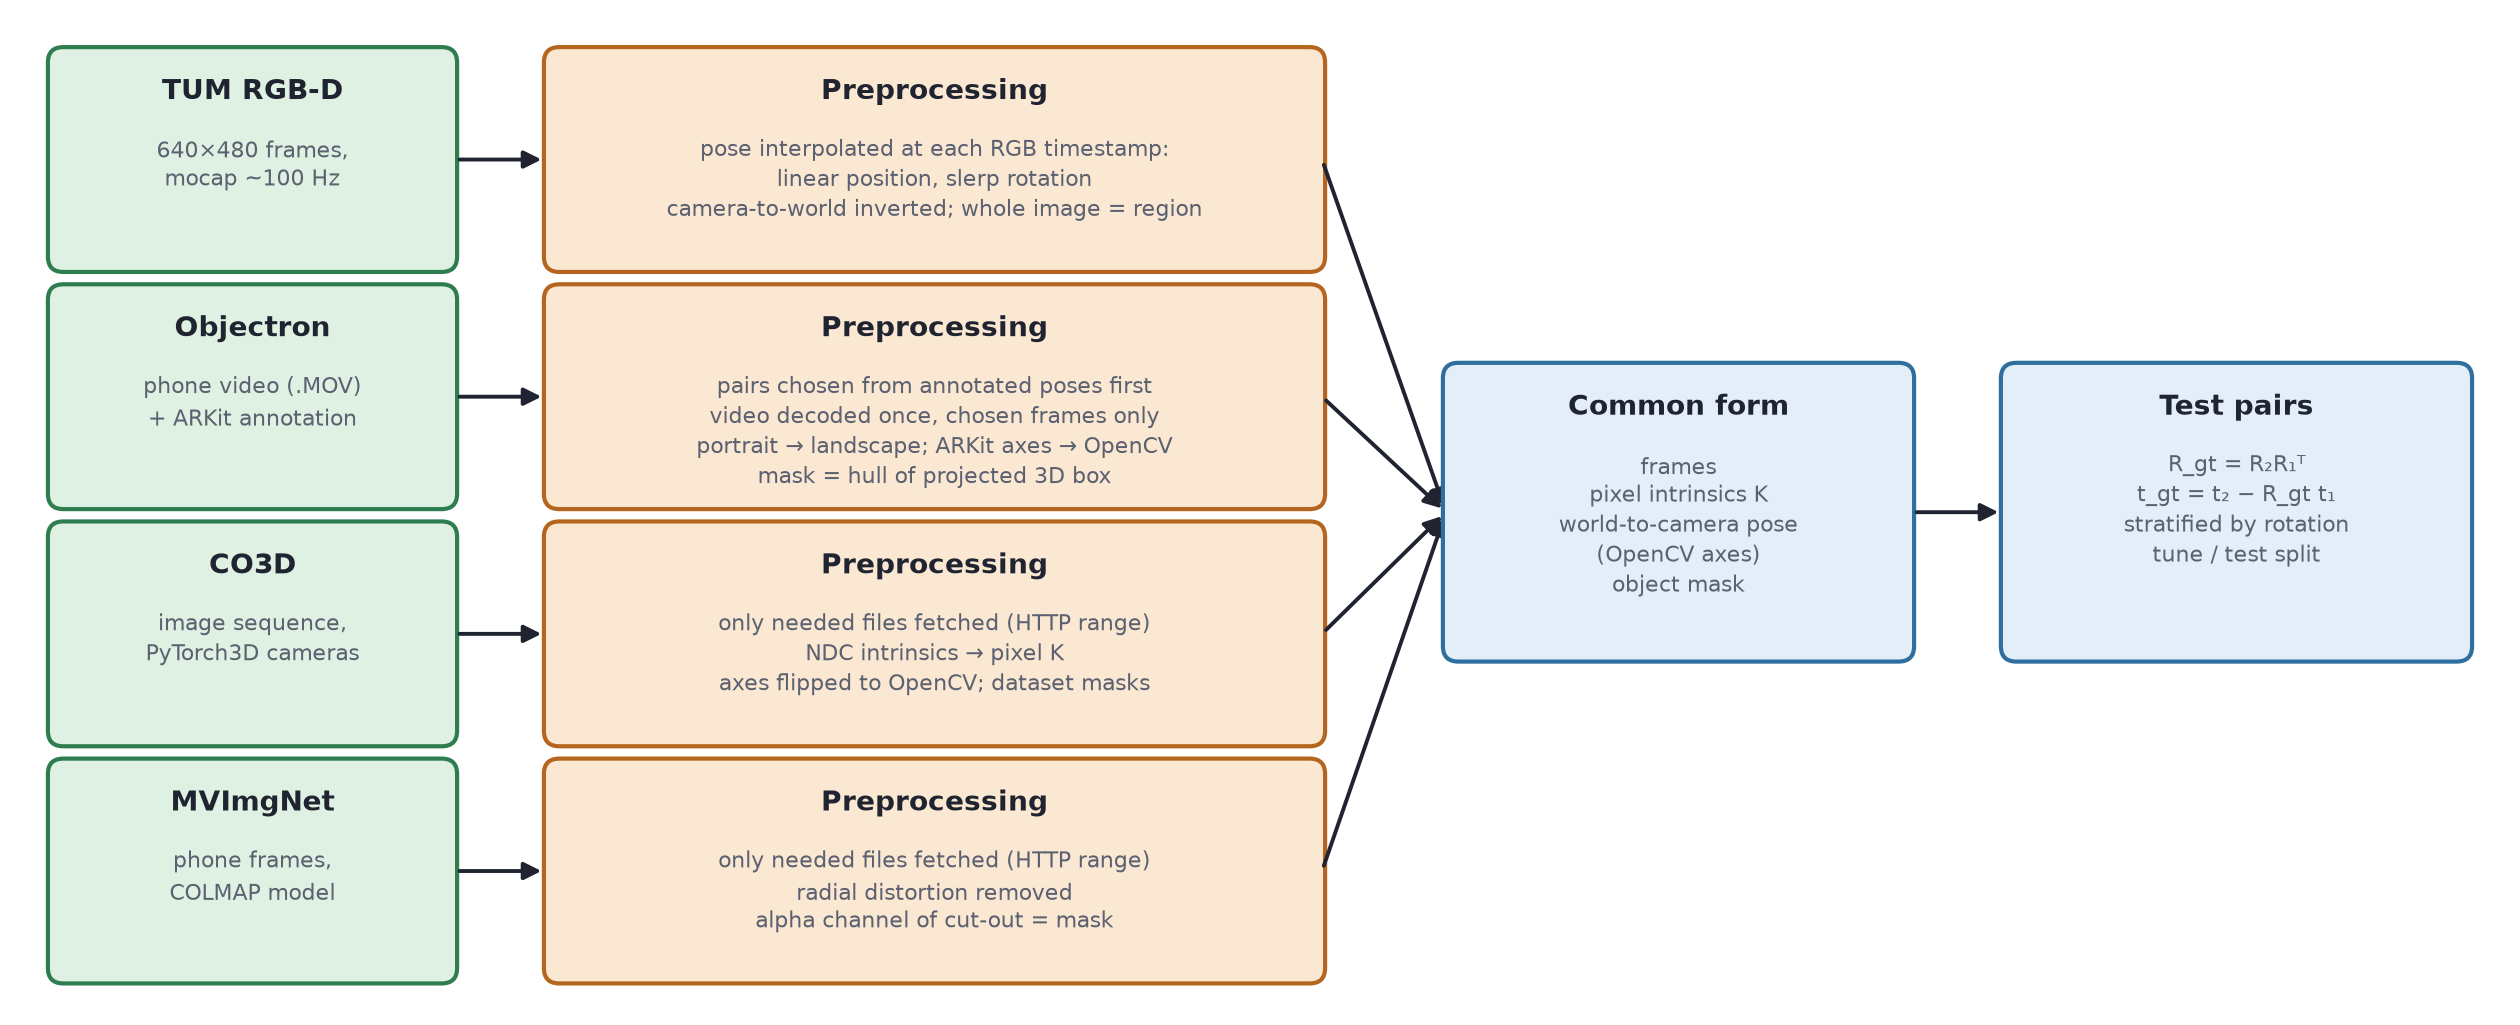
\includegraphics[width=0.9\textwidth]{dataprep.png}
  \caption{Offline preparation of the evaluation data: each dataset is converted to frames with pixel intrinsics, an OpenCV world-to-camera pose and an object mask, from which the test pairs and their ground-truth relative poses are formed.}
  \label{fig:dataprep}
\end{figure*}

\subsection*{Camera Model and Focal-Length Estimation}
A point $\X=(X,Y,Z)^\top$ in camera coordinates projects to pixel $(u,v)$ through the pinhole model
\begin{gather}
  \lambda\,(u,v,1)^\top = \K\X,\\
  \K = \begin{pmatrix} f&0&c_x\\0&f&c_y\\0&0&1\end{pmatrix},
\end{gather}
so that a pixel determines only the ray $\x = \K^{-1}(u,v,1)^\top$. Square pixels, zero skew and a principal point at the image centre are assumed; the focal length $f$ is the only unknown.

The focal length is estimated from the point map predicted by MASt3R~\cite{mast3r} (described below), which assigns to every pixel $i$ of the first image a 3D point $(X_i,Y_i,Z_i)$ in that camera's frame. The pinhole model requires $(u_i-c_x,\,v_i-c_y)\approx f\,(X_i/Z_i,\,Y_i/Z_i)$, so every pixel provides an estimate of $f$. The estimates are combined robustly by minimising the sum of distances
\begin{equation}
  f^\star = \arg\min_f \sum_i \big\|\,\mathbf{p}_i - \mathbf{c} - f\,\mathbf{q}_i\big\|,
\end{equation}
where $\mathbf{q}_i = (X_i/Z_i,\,Y_i/Z_i)$ and $\mathbf{c}=(c_x,c_y)$. The minimum is found by Weiszfeld's iteratively reweighted least squares~\cite{weiszfeld,dust3r}. The network is run once for each ordering of the pair and the two estimates are averaged when the images have the same size. If the network is unavailable, a $70^\circ$ horizontal field of view is assumed and the result is flagged. On the test pairs the median focal-length error is 6\%.

\subsection*{Object Segmentation (SAM 2.1)}
SAM~2.1~\cite{sam,sam2} produces the mask of the object under a prompt. A hierarchical vision transformer (Hiera~\cite{hiera}) encodes the image once; for each prompt a light two-way transformer decoder, in which prompt tokens attend to image features and image features attend to the tokens, outputs the mask. Since no prompt is given, image~1 is prompted with a $12\times12$ grid of points. Near-duplicate masks (intersection over union above 0.8) are merged; masks touching the image border are treated as background, as are masks covering less than 0.2\% or more than 60\% of the image. The remaining segments are object candidates, ranked by area weighted by proximity to the image centre.

\subsection*{Identification of the Moved Object}
The object is taken to be the candidate whose motion between the images differs from that of the background.

\textbf{Background motion.} The full images are matched with XFeat~\cite{xfeat} and LightGlue~\cite{lightglue}. A fundamental matrix $F$, satisfying $\mathbf{p}_2^\top F\mathbf{p}_1=0$ for static points, is fitted to the matches outside all candidates with MAGSAC++~\cite{magsac}; it does not depend on the estimated focal length.

\textbf{Motion rule.} For each candidate the fraction of its matches whose Sampson distance to $F$ exceeds the threshold is compared with the same fraction for the background. A candidate with at least 8 matches, at least 1.5\% of the image, and an outlier fraction at least 50 percentage points above the background's has moved independently~\cite{torr}. When the background is a single plane, which leaves $F$ ambiguous, the test is repeated against an $F$ fitted to all matches.

\textbf{Change rule.} Specular or dark objects yield few matches. For these, a homography fitted to background matches near the candidate is used to warp image~1 onto image~2, cancelling the camera motion locally~\cite{irani}, and the normalised cross-correlation~\cite{lewis}
\begin{equation}
  \mathrm{NCC}(a,b) = \frac{\sum (a-\bar a)(b-\bar b)}{\sqrt{\sum (a-\bar a)^2\sum (b-\bar b)^2}}
\end{equation}
is computed inside the candidate and in a surrounding ring, allowing shifts of up to 12\,px. A candidate whose ring aligns (NCC $\ge 0.40$) while its interior is lower by at least 0.50 has moved. To prevent parallax and blur on small patches from being mistaken for motion, this rule alone is accepted only for segments covering at least 0.5\% of the image; both values were selected on the tuning split, where they raised AUC@10 from 65.8 to 77.6.

\textbf{Decision.} The largest candidate that moved is the object. If no candidate moved, either a large candidate that could not be judged is used (\emph{unconfirmed}), or the scene is static and the whole images are used (\emph{scene}); in a static scene the camera's motion relative to the scene equals its motion relative to the object. The corresponding segment in image~2 is the SAM segment that receives most of the object's matches.

\subsection*{Region-of-Interest Extraction}
Each image is cropped to the mask's bounding box enlarged by 20\% on each side and reduced to at most 800\,px on its longer side, so that a small object occupies most of the matcher's input. Matches outside the masks are discarded and the rest are mapped back to full-image coordinates; the intrinsic matrix is therefore unchanged, and the inlier threshold is scaled by the inverse of the resizing factor.

\subsection*{Feature Matching}
\textbf{MASt3R.} The default matcher is MASt3R~\cite{mast3r}, built on DUSt3R~\cite{dust3r}. Both images are encoded by a shared ViT-Large encoder; two transformer decoders exchange information through cross-attention at every block, and prediction heads output, for every pixel of both images, a 3D point in the first camera's frame, a confidence, and a local descriptor. The descriptors are trained with a contrastive (InfoNCE) objective on ground-truth correspondences. Matches are obtained as mutual nearest neighbours of the descriptors, starting from a grid with 8\,px spacing. Because correspondence is inferred from the predicted 3D structure of both views, the method is robust to large viewpoint changes and weak texture. Only the matches are used; the pose is computed geometrically as described below.

\textbf{Alternative matchers.} SIFT~\cite{sift} detects extrema of a difference-of-Gaussians scale space, assigns each a dominant orientation and describes it by 128 gradient-orientation histograms; it is invariant to scale and in-plane rotation, and matches are retained by Lowe's ratio test (0.75). XFeat~\cite{xfeat} is a lightweight convolutional detector-descriptor; LightGlue~\cite{lightglue} matches its keypoints with alternating self- and cross-attention and adaptive depth. LoFTR~\cite{loftr} is detector-free: coarse features at $1/8$ resolution are transformed by interleaved self- and cross-attention, matched by a dual softmax and refined to sub-pixel accuracy.

\textbf{Cascades.} Two presets trade accuracy for speed. \texttt{accurate} tries XFeat+LightGlue, an outline-based method for textureless rectangles, SIFT and LoFTR in turn, accepting the first with enough inliers (200, valid outline, 50, 120). \texttt{confident} tries XFeat+LightGlue, SIFT and the outline method, accepting a stage when a gradient-boosted classifier, trained on the tuning split from the inlier count, inlier ratio, reprojection error and GRIC difference, predicts a probability of at least 0.45 that the error is below $10^\circ$; otherwise MASt3R is used.

\subsection*{Robust Estimation of $H$ and $E$}
Two models are fitted to the correspondences with MAGSAC++~\cite{magsac}, which replaces RANSAC's single inlier threshold~\cite{ransac} by a marginalisation over noise scales and refines the best model by iteratively reweighted least squares. The homography,
\begin{equation}
  \mathbf{p}_2 \simeq H\mathbf{p}_1,\qquad H = \K_2\Big(\R + \frac{\tv\,\n^\top}{d}\Big)\K_1^{-1},
\end{equation}
is exact for a planar object with normal $\n$ at distance $d$ and is estimated from minimal samples of four correspondences by the direct linear transform~\cite{hz}. The essential matrix,
\begin{equation}
  \x_2^\top E\,\x_1 = 0,\qquad E = [\tv]_\times\R,
\end{equation}
holds for any rigid motion~\cite{longuethiggins} and is estimated from minimal samples of five normalised correspondences by Nist\'er's algorithm~\cite{nister}. The inlier threshold is 1.5\,px at matching resolution, divided by the focal length for $E$.

\subsection*{Model Selection}
Since $E$ generalises $H$, it fits at least as well even when the object is planar, so residuals alone cannot choose between them. The Geometric Robust Information Criterion~\cite{torr}
\begin{gather}
  \mathrm{GRIC} = \sum_i \rho\!\Big(\frac{e_i^2}{\sigma^2}\Big) + \lambda_1 d\,n + \lambda_2 k,\\
  \rho(x)=\min\!\big(x,\lambda_3(r-d)\big),
\end{gather}
penalises each model's freedom: $d$ is the dimension of the model's manifold in the four-dimensional space of correspondences ($d=2$ for $H$, $d=3$ for $E$), $k$ the number of parameters (8 and 5), $r=4$, $\lambda_1=\ln r$, $\lambda_2=\ln rn$ and $\lambda_3=2$. Residuals $e_i$ are the symmetric transfer error for $H$ and the Sampson distance for $E$. The model with the lower score is used.

\subsection*{Pose Decomposition}
\textbf{From $E$.} With $E=U\,\mathrm{diag}(1,1,0)\,V^\top$, the four candidates are $\R\in\{UWV^\top, UW^\top V^\top\}$ and $\tv=\pm\mathbf{u}_3$~\cite{hz}; the candidate placing the triangulated points in front of both cameras is retained.

\textbf{From $H$.} The normalised homography $\K_2^{-1}H\K_1=\R+\tv\n^\top/d$ is decomposed into up to four solutions~\cite{malis}, of which two remain after the visibility test. For a planar scene both reproduce the images exactly~\cite{faugeras}. They are separated by the number of points in front of both cameras, then by the median Sampson error over all correspondences---points slightly off the plane are explained only by the true pose---when one candidate is better by a factor of 1.5, and otherwise by the prior that the plane faces both cameras.

\textbf{Planar-twin check.} When $E$ is selected for a nearly planar object, it can coincide with the incorrect plane solution. If the pose from $E$ lies within $10^\circ$ of one candidate of the homography decomposition, the other candidate replaces it when it explains all correspondences nearly as well (median Sampson error within a factor of 3) and the evidence above prefers it.

\subsection*{Non-linear Refinement}
The pose is refined over all inliers by Levenberg--Marquardt~\cite{levenberg,marquardt}. For $E$ the parameters are the rotation (three, as a rotation vector) and the translation direction (two, on the unit sphere), and the residual is the Sampson distance. For $H$ they are the rotation, the translation scaled by the inverse plane distance and the plane normal (eight in total), and the residual is the symmetric transfer error of the induced homography. The refined pose is kept only if the median residual decreases; inliers are then re-selected among all correspondences and the refinement repeated once.

\subsection*{Reprojection Error and Verdict}
The inliers are triangulated with the final pose, and points in front of both cameras are projected back into both images. The reported reprojection error is
\begin{equation}
  \epsilon_{\mathrm{RMS}} = \sqrt{\frac{1}{2N}\sum_{i=1}^{N}\Big(\|\hat{\mathbf{p}}_{1,i}-\mathbf{p}_{1,i}\|^2+\|\hat{\mathbf{p}}_{2,i}-\mathbf{p}_{2,i}\|^2\Big)} .
\end{equation}
This quantity measures the consistency of the pose with the inliers but not its correctness, since an incorrect but self-consistent solution attains a similar value. A verdict is therefore attached: \textsc{uncertain} for fewer than 30 inliers, an error above 2\,px, a rotation above $60^\circ$ with a 2D matcher, or an assumed focal length; \textsc{scene motion only} when the whole images were used; \textsc{reliable} otherwise. If the pose cannot be computed from an automatically found region, it is recomputed from the whole images.

\subsection*{Evaluation Against Ground Truth}
The rotation error is the geodesic angle and the translation error the angle between directions:
\begin{align}
  e_R &= \arccos\!\Big(\tfrac{\mathrm{tr}(\R_{est}^\top\R_{gt})-1}{2}\Big),\\
  e_t &= \arccos\!\Big(\tfrac{\tv_{est}^\top\tv_{gt}}{\|\tv_{est}\|\,\|\tv_{gt}\|}\Big).
\end{align}
The pose error is $\max(e_R,e_t)$. The area under the cumulative pose-error curve up to $\tau\in\{5^\circ,10^\circ,20^\circ\}$, normalised to 100 (AUC@$\tau$), is reported as in~\cite{superglue,loftr}, with failures counted as infinite error. For comparability with earlier coursework, the rotation is also expressed as roll $=\mathrm{atan2}(r_{32},r_{33})$, pitch $=-\arcsin r_{31}$ and yaw $=\mathrm{atan2}(r_{21},r_{11})$, and per-axis absolute errors are summarised by MAE, MSE, maximum, minimum and standard deviation.

% ------------------------------------------------------------------ 3
\section{Results}

\subsection{Worked Example}
Figure~\ref{fig:case-planar} follows one test pair through every stage: a planar poster scene from TUM with $22.0^\circ$ of rotation. SAM~2.1 returns several candidate segments (panel~2); all of them follow the background's epipolar geometry (panel~3) and align after the background motion is removed (panel~4), so the scene is classified as static and the whole images are used. MASt3R provides dense correspondences; GRIC selects the model, and the decomposed and refined pose has a rotation error of $1.68^\circ$ with a reprojection error of 0.17\,px. The estimated focal length is used throughout; no ground-truth quantity enters the computation.

\begin{figure*}[p]
  \centering
  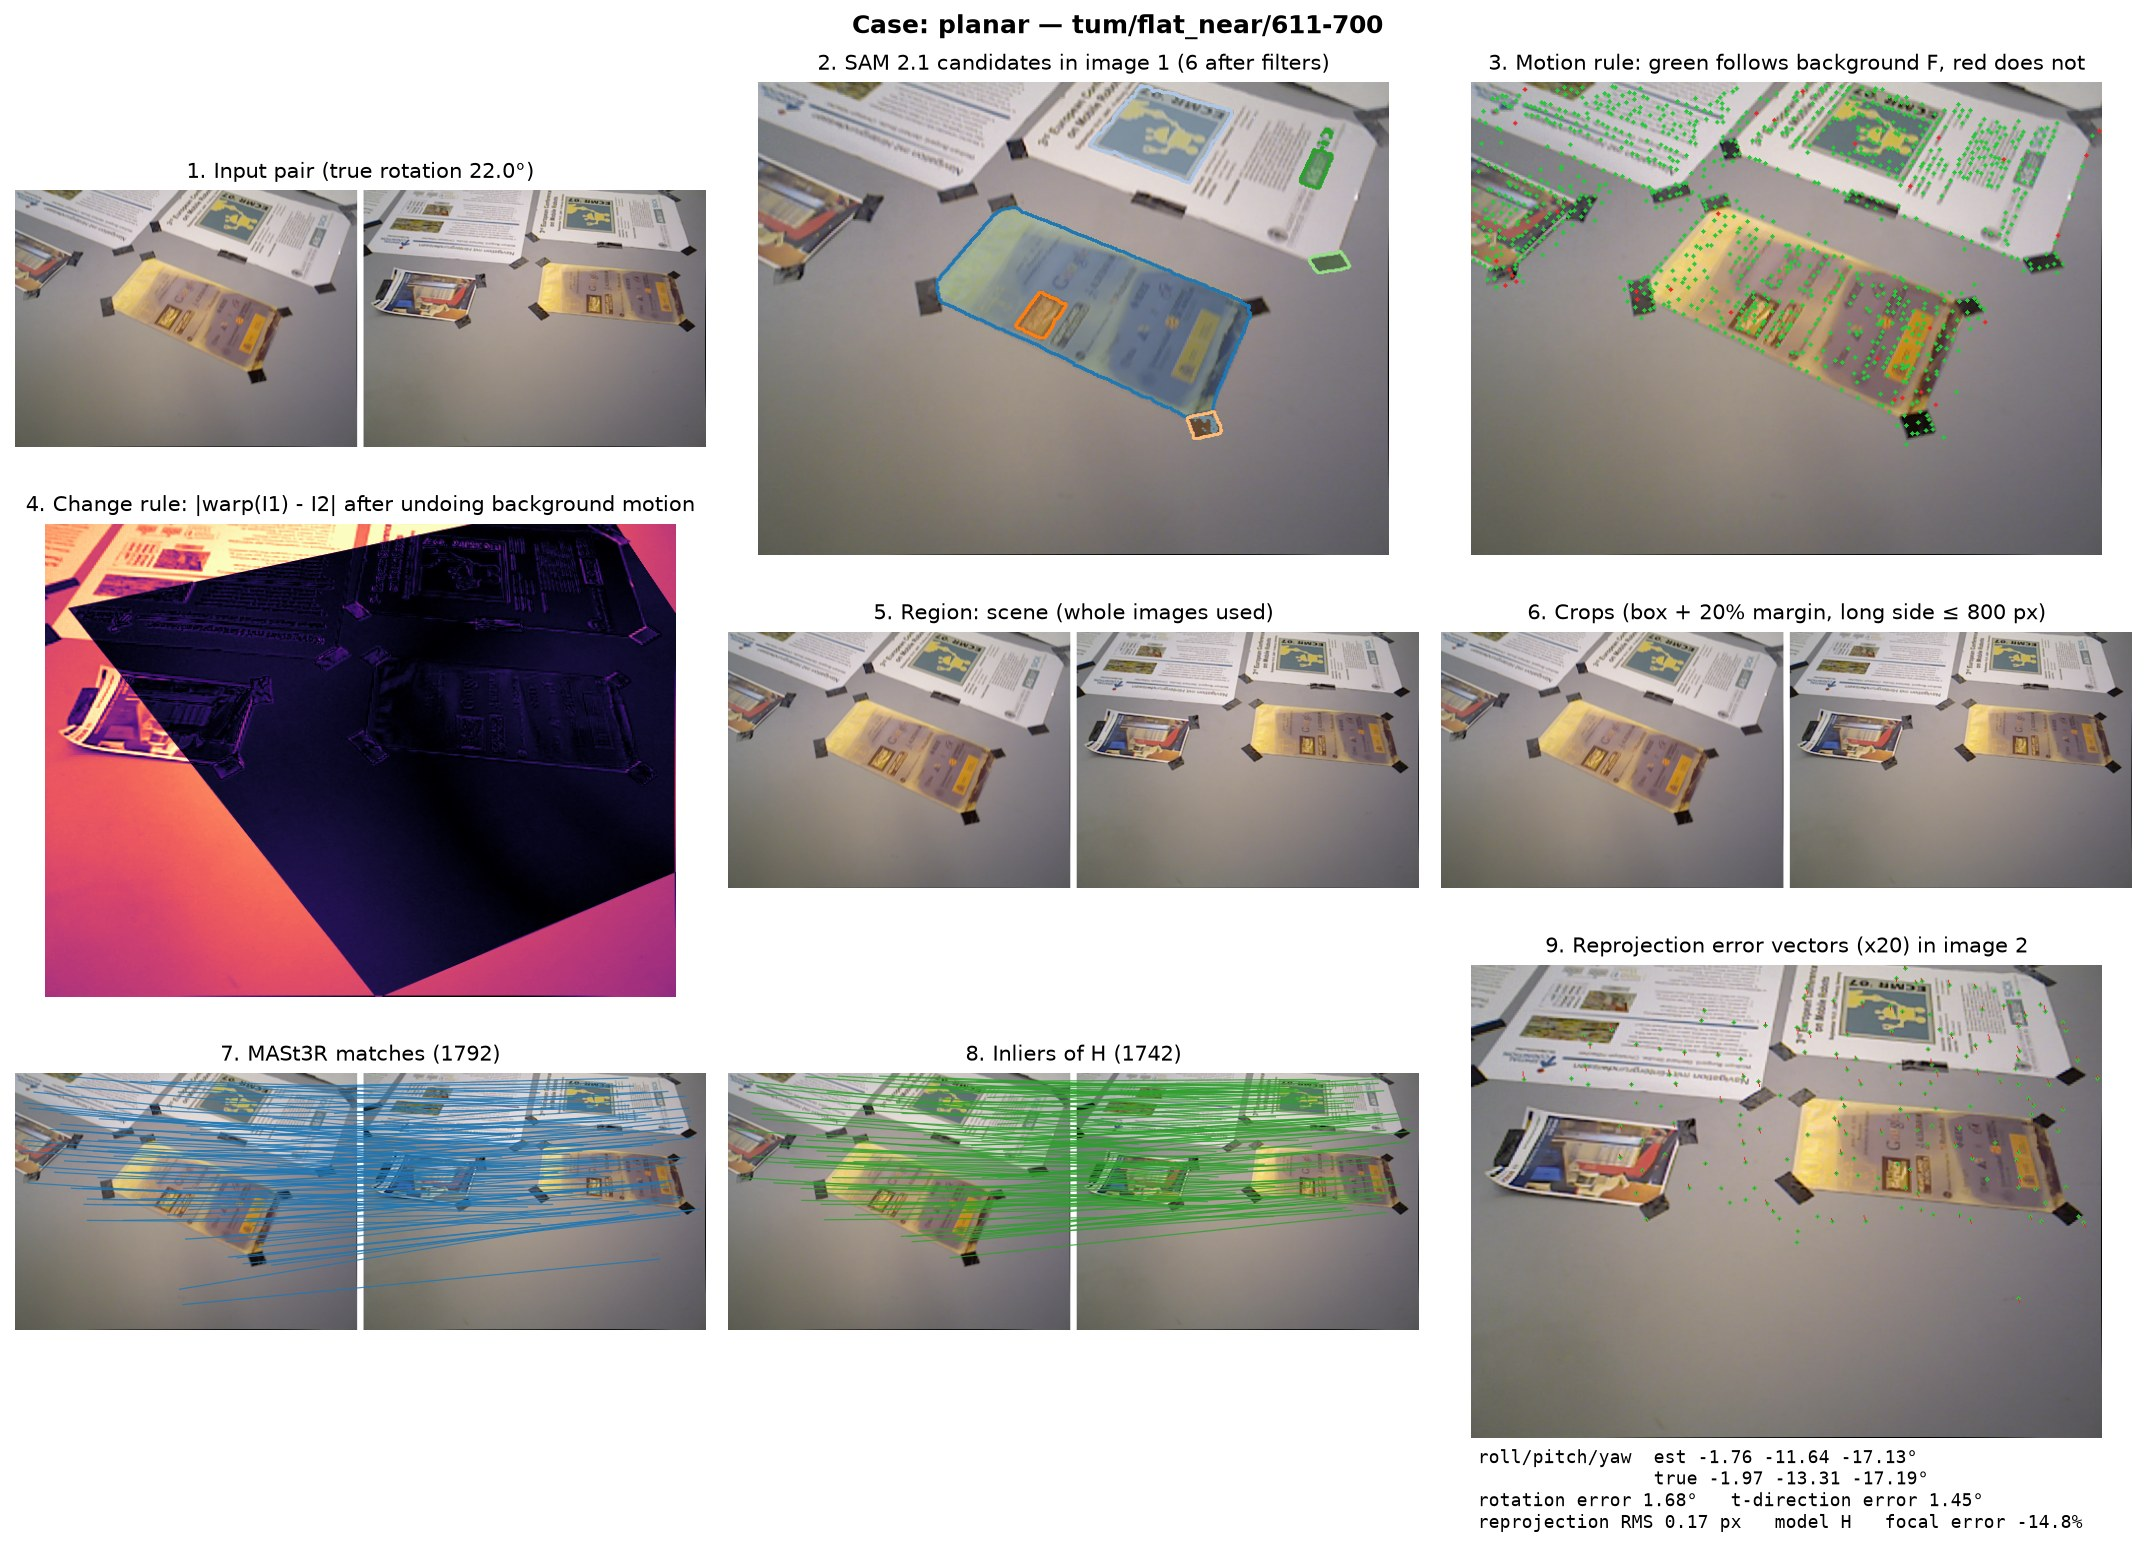
\includegraphics[width=\textwidth]{case_planar.jpg}
  \caption{Worked example (TUM poster, $22.0^\circ$): input, SAM~2.1 candidates, motion rule, change rule, region, crops, MASt3R matches, inliers of the selected model, and reprojection error vectors (magnified $20\times$) with the errors against ground truth.}
  \label{fig:case-planar}
\end{figure*}

\subsection{Quantitative Results}
Table~\ref{tab:main} summarises the 56 test pairs. With only the two images, MASt3R attains AUC@10 of 57.5, against 58.5 for the same estimator given the dataset's intrinsics and object region; estimating the focal length and finding the object therefore cost one point on average. The \texttt{confident} cascade is within 2.4 points at a small fraction of the matching time, whereas \texttt{accurate}, which relies on 2D matchers only, loses 18 points.

\begin{table}[H]
\centering\small\setlength{\tabcolsep}{3pt}
\resizebox{\columnwidth}{!}{%
\begin{tabular}{lccccc}
\toprule
Method & AUC@5/10/20 & $\tilde e_R$ & $\tilde e_t$ & $\tilde\epsilon$ (px) & $>20^\circ$\\
\midrule
MASt3R & 41.4 / \textbf{57.5} / 68.9 & \textbf{0.97}$^\circ$ & 1.79$^\circ$ & \textbf{0.46} & 18\%\\
\texttt{confident} & 40.5 / 55.2 / 65.7 & 1.07$^\circ$ & \textbf{1.74}$^\circ$ & 0.63 & 23\%\\
\texttt{accurate} & 30.7 / 39.8 / 47.3 & 1.57$^\circ$ & 7.79$^\circ$ & 0.77 & 45\%\\
\midrule
\emph{Reference} & 44.4 / 58.5 / 69.7 & 0.72$^\circ$ & 2.20$^\circ$ & 0.32 & 18\%\\
\bottomrule
\end{tabular}}
\caption{Results on 56 test pairs using only the two images; $\tilde{\cdot}$ denotes the median. \emph{Reference}: MASt3R with the dataset intrinsics and object region.}
\label{tab:main}
\end{table}

\begin{table}[H]
\centering\small\setlength{\tabcolsep}{3pt}
\resizebox{\columnwidth}{!}{%
\begin{tabular}{lcccccc}
\toprule
Viewpoint & $n$ & MASt3R & \texttt{conf.} & \texttt{acc.} & $\tilde e_R$ & $\tilde e_t$\\
\midrule
$<1^\circ$ (consecutive) & 10 & 7.4 & 7.4 & 0.0 & 0.32$^\circ$ & 44.6$^\circ$\\
5--15$^\circ$ & 12 & 70.9 & 72.3 & 68.2 & 0.76$^\circ$ & 1.65$^\circ$\\
15--30$^\circ$ & 11 & 80.3 & 71.3 & 71.3 & 1.11$^\circ$ & 0.78$^\circ$\\
30--60$^\circ$ & 9 & 68.8 & 59.5 & 53.0 & 1.68$^\circ$ & 1.77$^\circ$\\
60--90$^\circ$ & 14 & 65.2 & 67.8 & 17.2 & 3.08$^\circ$ & 1.41$^\circ$\\
\bottomrule
\end{tabular}}
\caption{AUC@10 by viewpoint change; median errors are for MASt3R.}
\label{tab:views}
\end{table}

Table~\ref{tab:views} and Figure~\ref{fig:viewpoint} show the dependence on viewpoint change. Between $5^\circ$ and $90^\circ$ the median rotation error of MASt3R grows from $0.76^\circ$ to $3.08^\circ$, while the 2D cascade fails on most pairs beyond $60^\circ$. On consecutive frames the rotation is accurate ($0.32^\circ$) but the translation direction is not observable, because the baseline is a few millimetres; since the pose error is the larger of the two errors, AUC is low for every method in this regime. Figure~\ref{fig:cdf} gives the cumulative distribution of the pose error.

\begin{figure}[H]
  \centering
  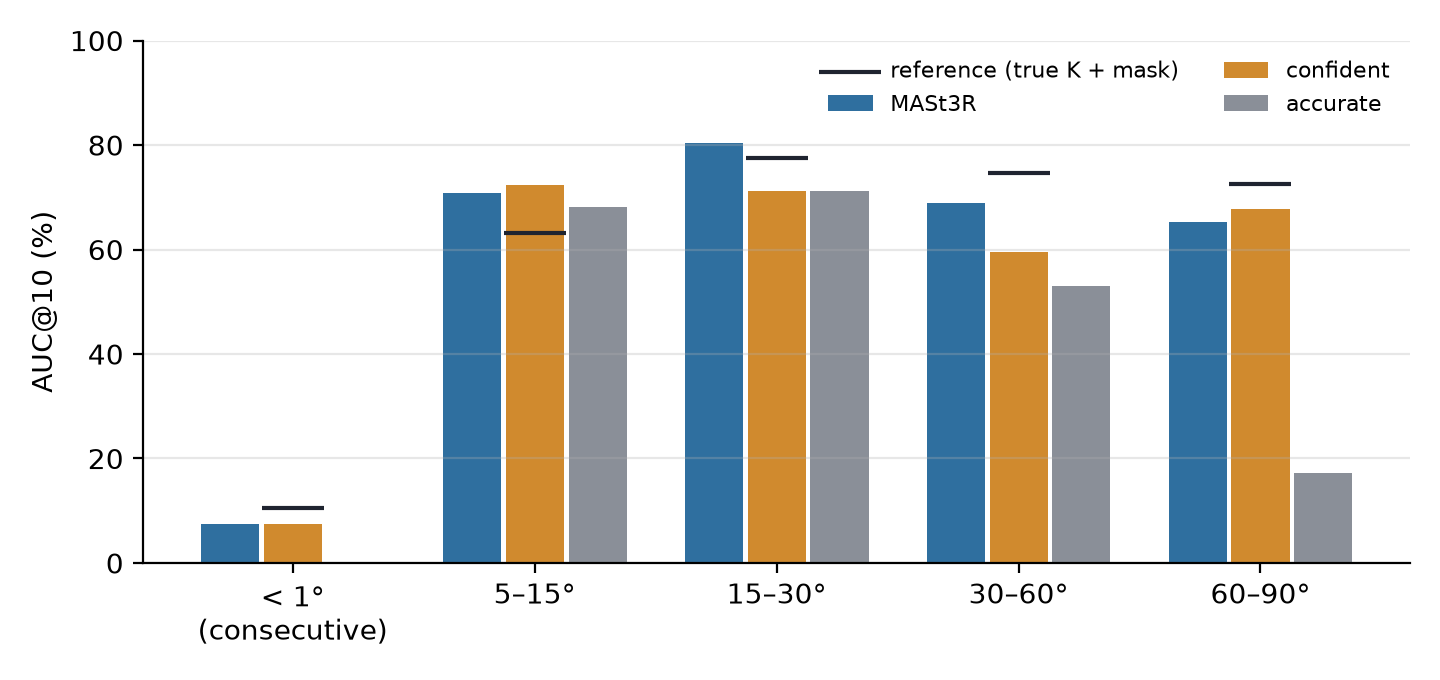
\includegraphics[width=\columnwidth]{viewpoint.png}
  \caption{AUC@10 by viewpoint change. Bars: two images only; ticks: reference with true intrinsics and object region.}
  \label{fig:viewpoint}
\end{figure}

\begin{figure}[H]
  \centering
  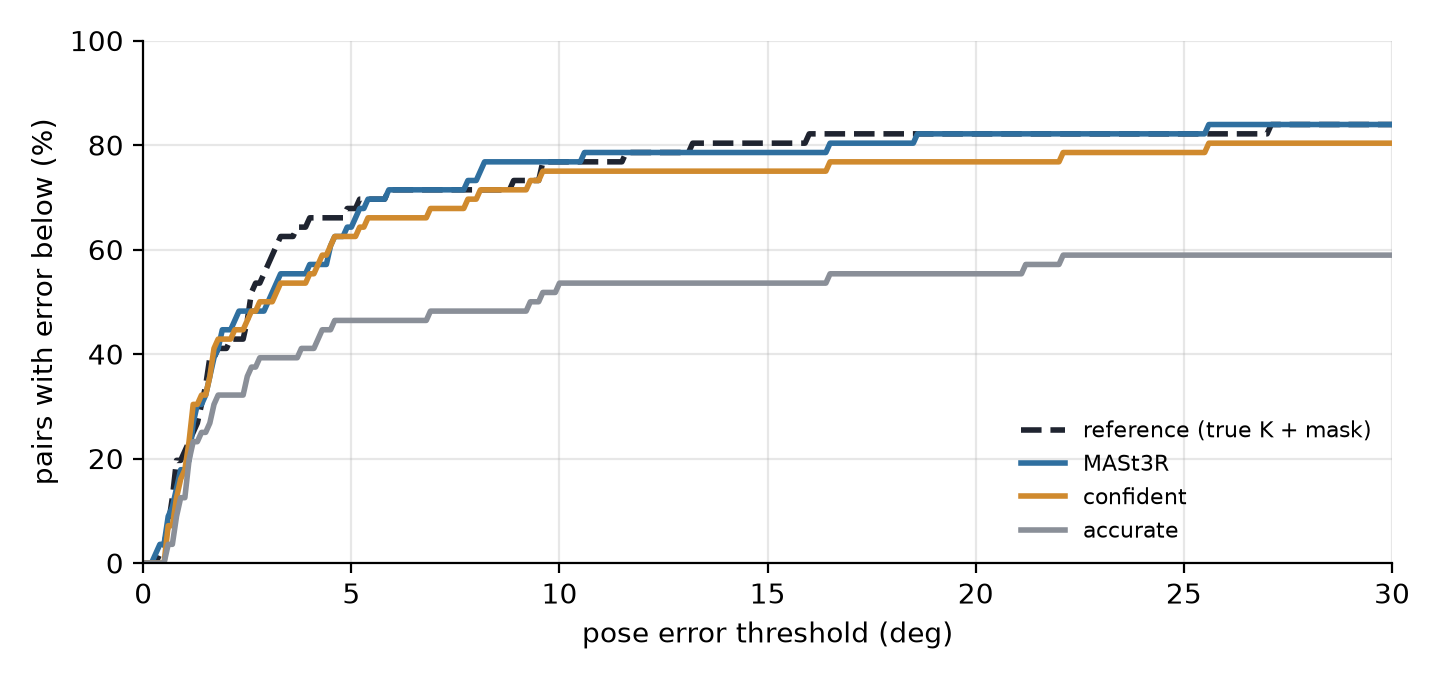
\includegraphics[width=\columnwidth]{cdf.png}
  \caption{Fraction of test pairs whose pose error is below a threshold.}
  \label{fig:cdf}
\end{figure}

\textbf{Error statistics.} Tables~\ref{tab:global-small} and~\ref{tab:global-track} report the error statistics in the format of per-axis and global metrics for two regimes: consecutive frames, and pairs 20 frames apart along a TUM sequence (rotations of $1$--$12^\circ$), each solved from the two images only.

\begin{table}[H]
\centering\small\setlength{\tabcolsep}{3pt}
\resizebox{\columnwidth}{!}{%
\begin{tabular}{lcccccc}
\toprule
Metric & MAE & MSE & MAX & MIN & STD & $n$\\
\midrule
\multicolumn{7}{l}{\textit{Global metrics}}\\
Rotation error, avg.\ axis (deg) & 0.195 & 0.047 & 0.368 & 0.039 & 0.094 & 10\\
Rotation error, geodesic (deg) & 0.400 & 0.202 & 0.762 & 0.078 & 0.205 & 10\\
Translation direction (deg) & 48.05 & 3395 & 113.8 & 5.20 & 32.96 & 10\\
Reprojection RMS (px) & 0.221 & 0.050 & 0.270 & 0.186 & 0.028 & 10\\
\multicolumn{7}{l}{\textit{Per-axis absolute error (deg)}}\\
Roll & 0.248 & 0.094 & 0.683 & 0.000 & 0.181 & 10\\
Pitch & 0.124 & 0.023 & 0.326 & 0.016 & 0.088 & 10\\
Yaw & 0.215 & 0.085 & 0.684 & 0.016 & 0.197 & 10\\
\bottomrule
\end{tabular}}
\caption{Consecutive frames (small-motion regime), MASt3R, two images only.}
\label{tab:global-small}
\end{table}

\begin{table}[H]
\centering\small\setlength{\tabcolsep}{3pt}
\resizebox{\columnwidth}{!}{%
\begin{tabular}{lcccccc}
\toprule
Metric & MAE & MSE & MAX & MIN & STD & $n$\\
\midrule
\multicolumn{7}{l}{\textit{Global metrics}}\\
Rotation error, avg.\ axis (deg) & 0.316 & 0.419 & 3.478 & 0.034 & 0.565 & 38\\
Rotation error, geodesic (deg) & 0.700 & 2.536 & 8.662 & 0.060 & 1.430 & 38\\
Translation direction (deg) & 8.439 & 196.5 & 57.67 & 0.837 & 11.20 & 38\\
Reprojection RMS (px) & 0.211 & 0.047 & 0.327 & 0.044 & 0.046 & 38\\
\multicolumn{7}{l}{\textit{Per-axis absolute error (deg)}}\\
Roll & 0.426 & 1.953 & 8.482 & 0.005 & 1.331 & 38\\
Pitch & 0.337 & 0.529 & 3.838 & 0.008 & 0.645 & 38\\
Yaw & 0.187 & 0.055 & 0.751 & 0.021 & 0.142 & 38\\
\bottomrule
\end{tabular}}
\caption{TUM \texttt{struct\_near}, pairs 20 frames apart (larger-motion regime), MASt3R, two images only.}
\label{tab:global-track}
\end{table}

\begin{figure*}[t]
  \centering
  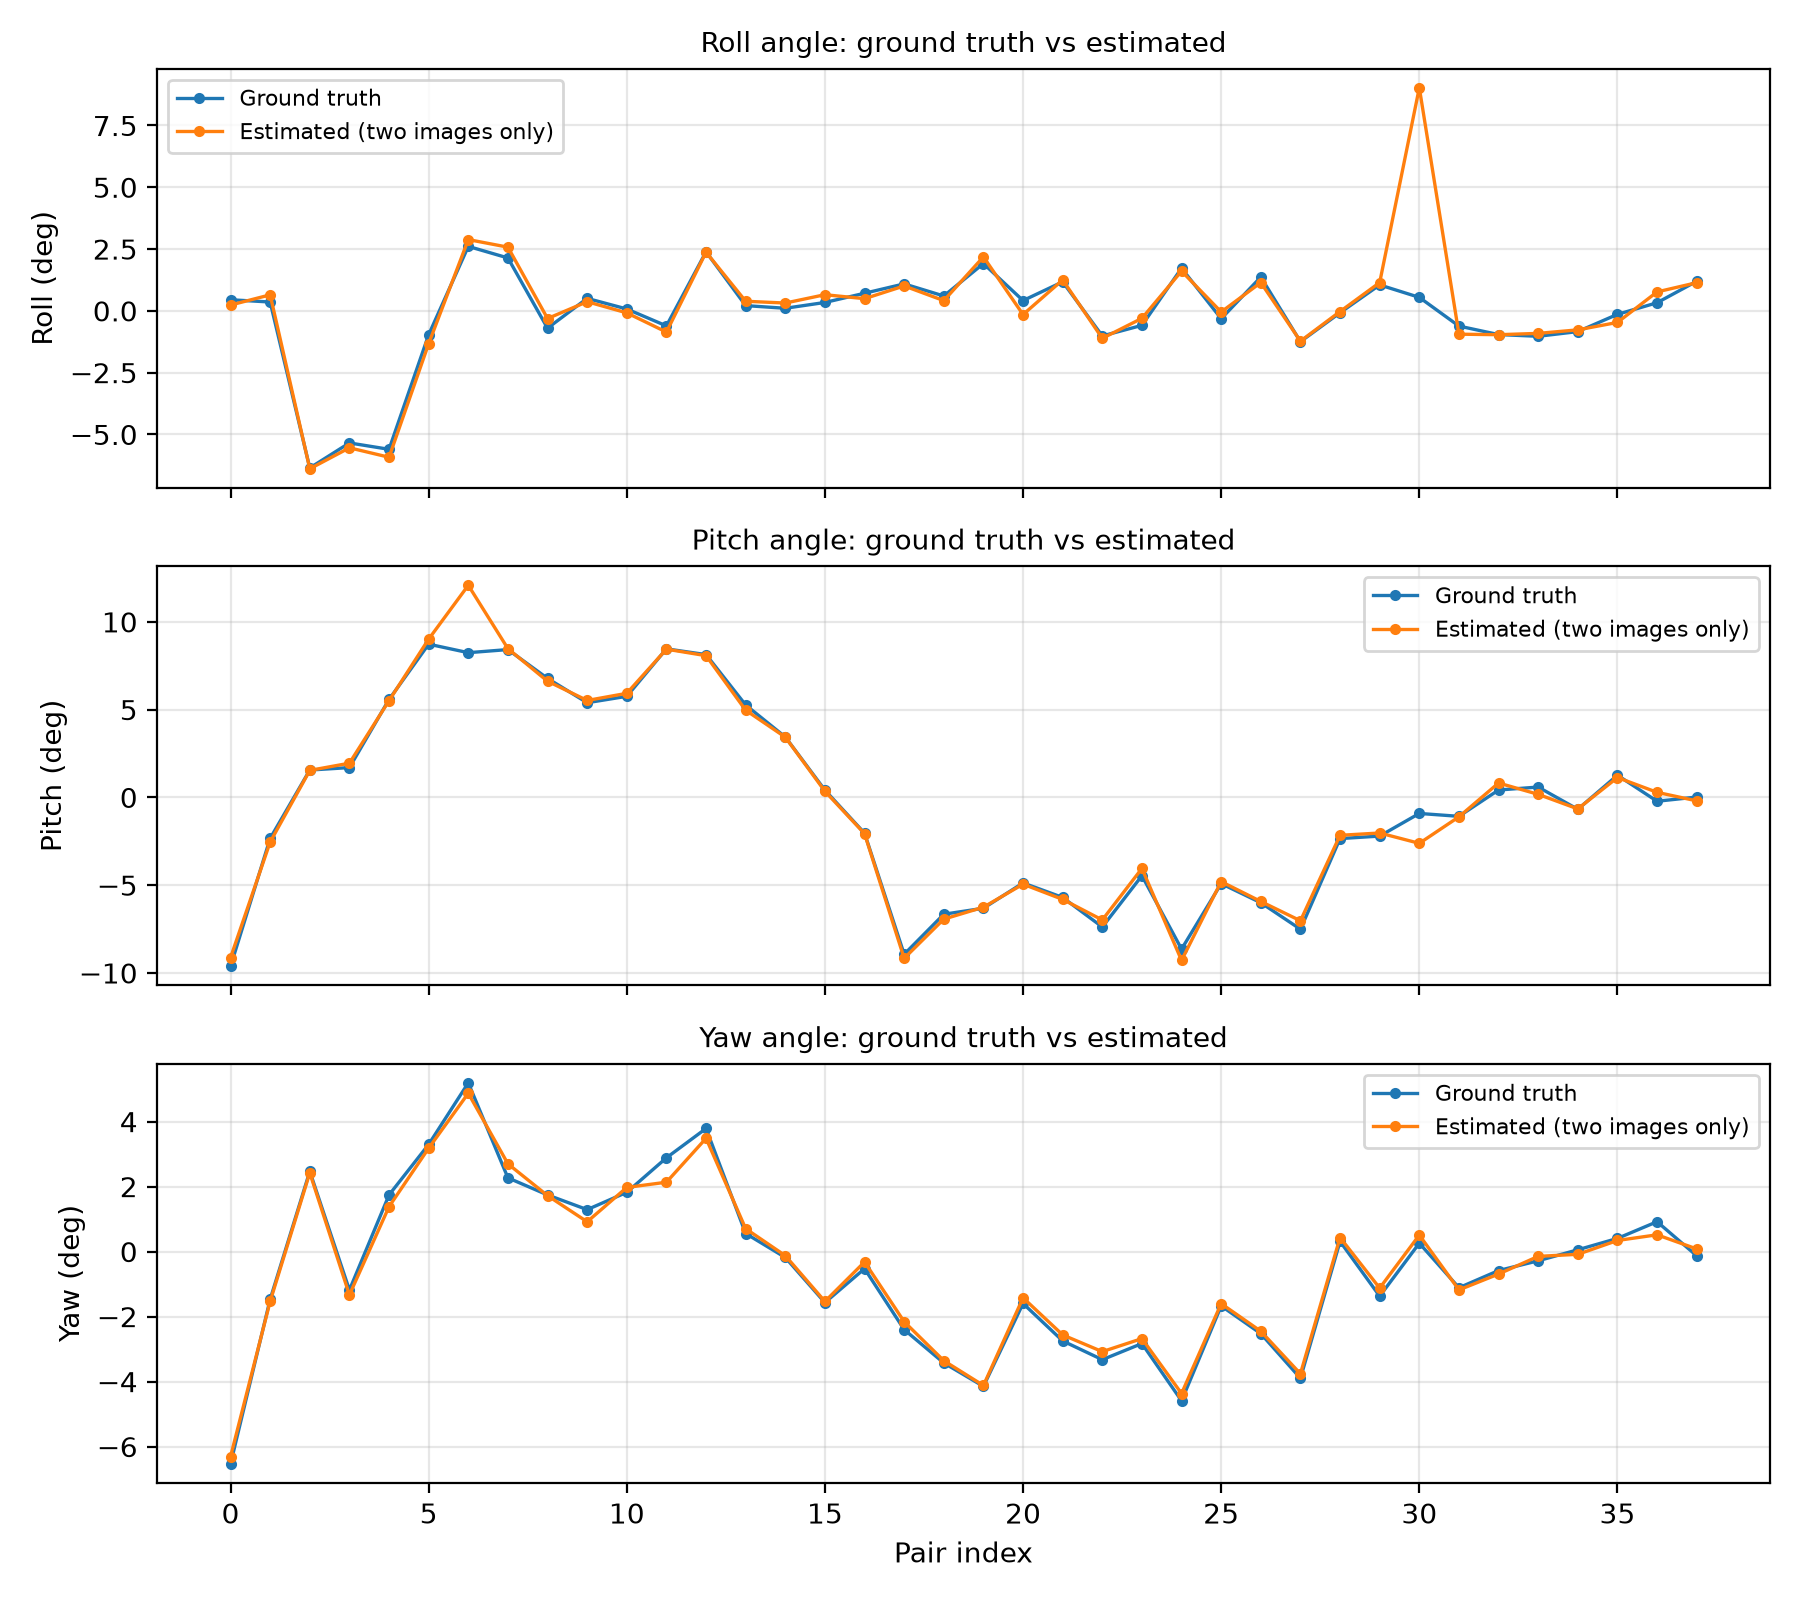
\includegraphics[width=0.86\textwidth]{euler_struct_near_gap20.png}
  \caption{Frame-wise roll, pitch and yaw against ground truth for 38 consecutive pairs 20 frames apart (TUM \texttt{struct\_near}), each estimated from the two images only. The estimates follow the ground truth closely; the largest deviations are a roll error of $8.5^\circ$ at pair 30 and a pitch overshoot of $3.8^\circ$ at pair 6.}
  \label{fig:euler}
\end{figure*}

\subsection{Planar and Non-planar Objects}
On the 32 pairs of near-planar objects MASt3R reaches AUC@10 of 56.1 and on the 24 three-dimensional pairs 61.1, so the planar case is handled nearly as well as the general one. The 2D cascade degrades much more on planar objects (32.5 against 51.5).

\subsection{Effect of the Region Rule}
The minimum segment size and stronger contrast required of the change rule were introduced after observing that, in static scenes, small patches were misclassified as moved. On the same 56 test pairs this change, selected on the tuning split, raised AUC@10 of MASt3R from 50.2 to 57.5, reduced the median rotation error from $1.27^\circ$ to $0.97^\circ$ and the share of pairs above $20^\circ$ from 25\% to 18\%.

\subsection{Comparison of Matchers}
Table~\ref{tab:six} compares all six methods on the 46 test pairs with appreciable motion (the consecutive-frame pairs are excluded, since their translation direction is not observable). Every method receives the same estimated focal length and the same automatically found region. MASt3R is the most accurate and never fails; the confidence-gated cascade is second, and the three 2D matchers are close to one another, failing on 9--26\% of pairs.

\begin{table}[H]
\centering\small\setlength{\tabcolsep}{3pt}
\resizebox{\columnwidth}{!}{%
\begin{tabular}{lccccc}
\toprule
Method & AUC@5/10/20 & $\tilde e_R$ & $\tilde e_t$ & $>20^\circ$ & failed\\
\midrule
SIFT & 33.4 / 46.4 / 55.3 & 1.77$^\circ$ & 3.81$^\circ$ & 35\% & 26\%\\
XFeat+LightGlue & 35.7 / 46.6 / 56.9 & 3.44$^\circ$ & 1.81$^\circ$ & 33\% & 13\%\\
LoFTR & 35.3 / 46.7 / 55.4 & 2.36$^\circ$ & 2.59$^\circ$ & 35\% & 9\%\\
MASt3R & \textbf{50.4} / \textbf{69.0} / \textbf{81.0} & \textbf{1.17}$^\circ$ & \textbf{1.39}$^\circ$ & \textbf{7\%} & 0\%\\
\midrule
\texttt{accurate} & 37.3 / 48.5 / 56.8 & 2.47$^\circ$ & 1.82$^\circ$ & 35\% & 0\%\\
\texttt{confident} & 49.3 / 66.1 / 77.6 & 1.44$^\circ$ & 1.43$^\circ$ & 11\% & 0\%\\
\bottomrule
\end{tabular}}
\caption{All six methods on 46 test pairs ($\ge 5^\circ$), two images only.}
\label{tab:six}
\end{table}

Figure~\ref{fig:methods} shows, for individual pairs, situations in which a particular method gives clearly the best pose, together with the result of every method on the same pair. A pair is shown for a method only if its pose error is at most $5^\circ$ and every other method is at least twice and $3^\circ$ worse; a cascade is credited when it selects a stage that succeeds while the methods it did not select fail. MASt3R succeeds on keys with weak texture where the 2D matchers fail; \texttt{confident} succeeds on a similar pair by deferring to MASt3R; \texttt{accurate} succeeds on a laptop through its outline-based stage when every correspondence-based method is $8$--$12^\circ$ in error; and LoFTR succeeds on the checkerboard pair of Figure~\ref{fig:failure}, where MASt3R's correspondences between the incorrectly paired regions lead to a large error. No pair satisfied the criterion for SIFT or XFeat+LightGlue alone.

\begin{figure*}[t]
  \centering
  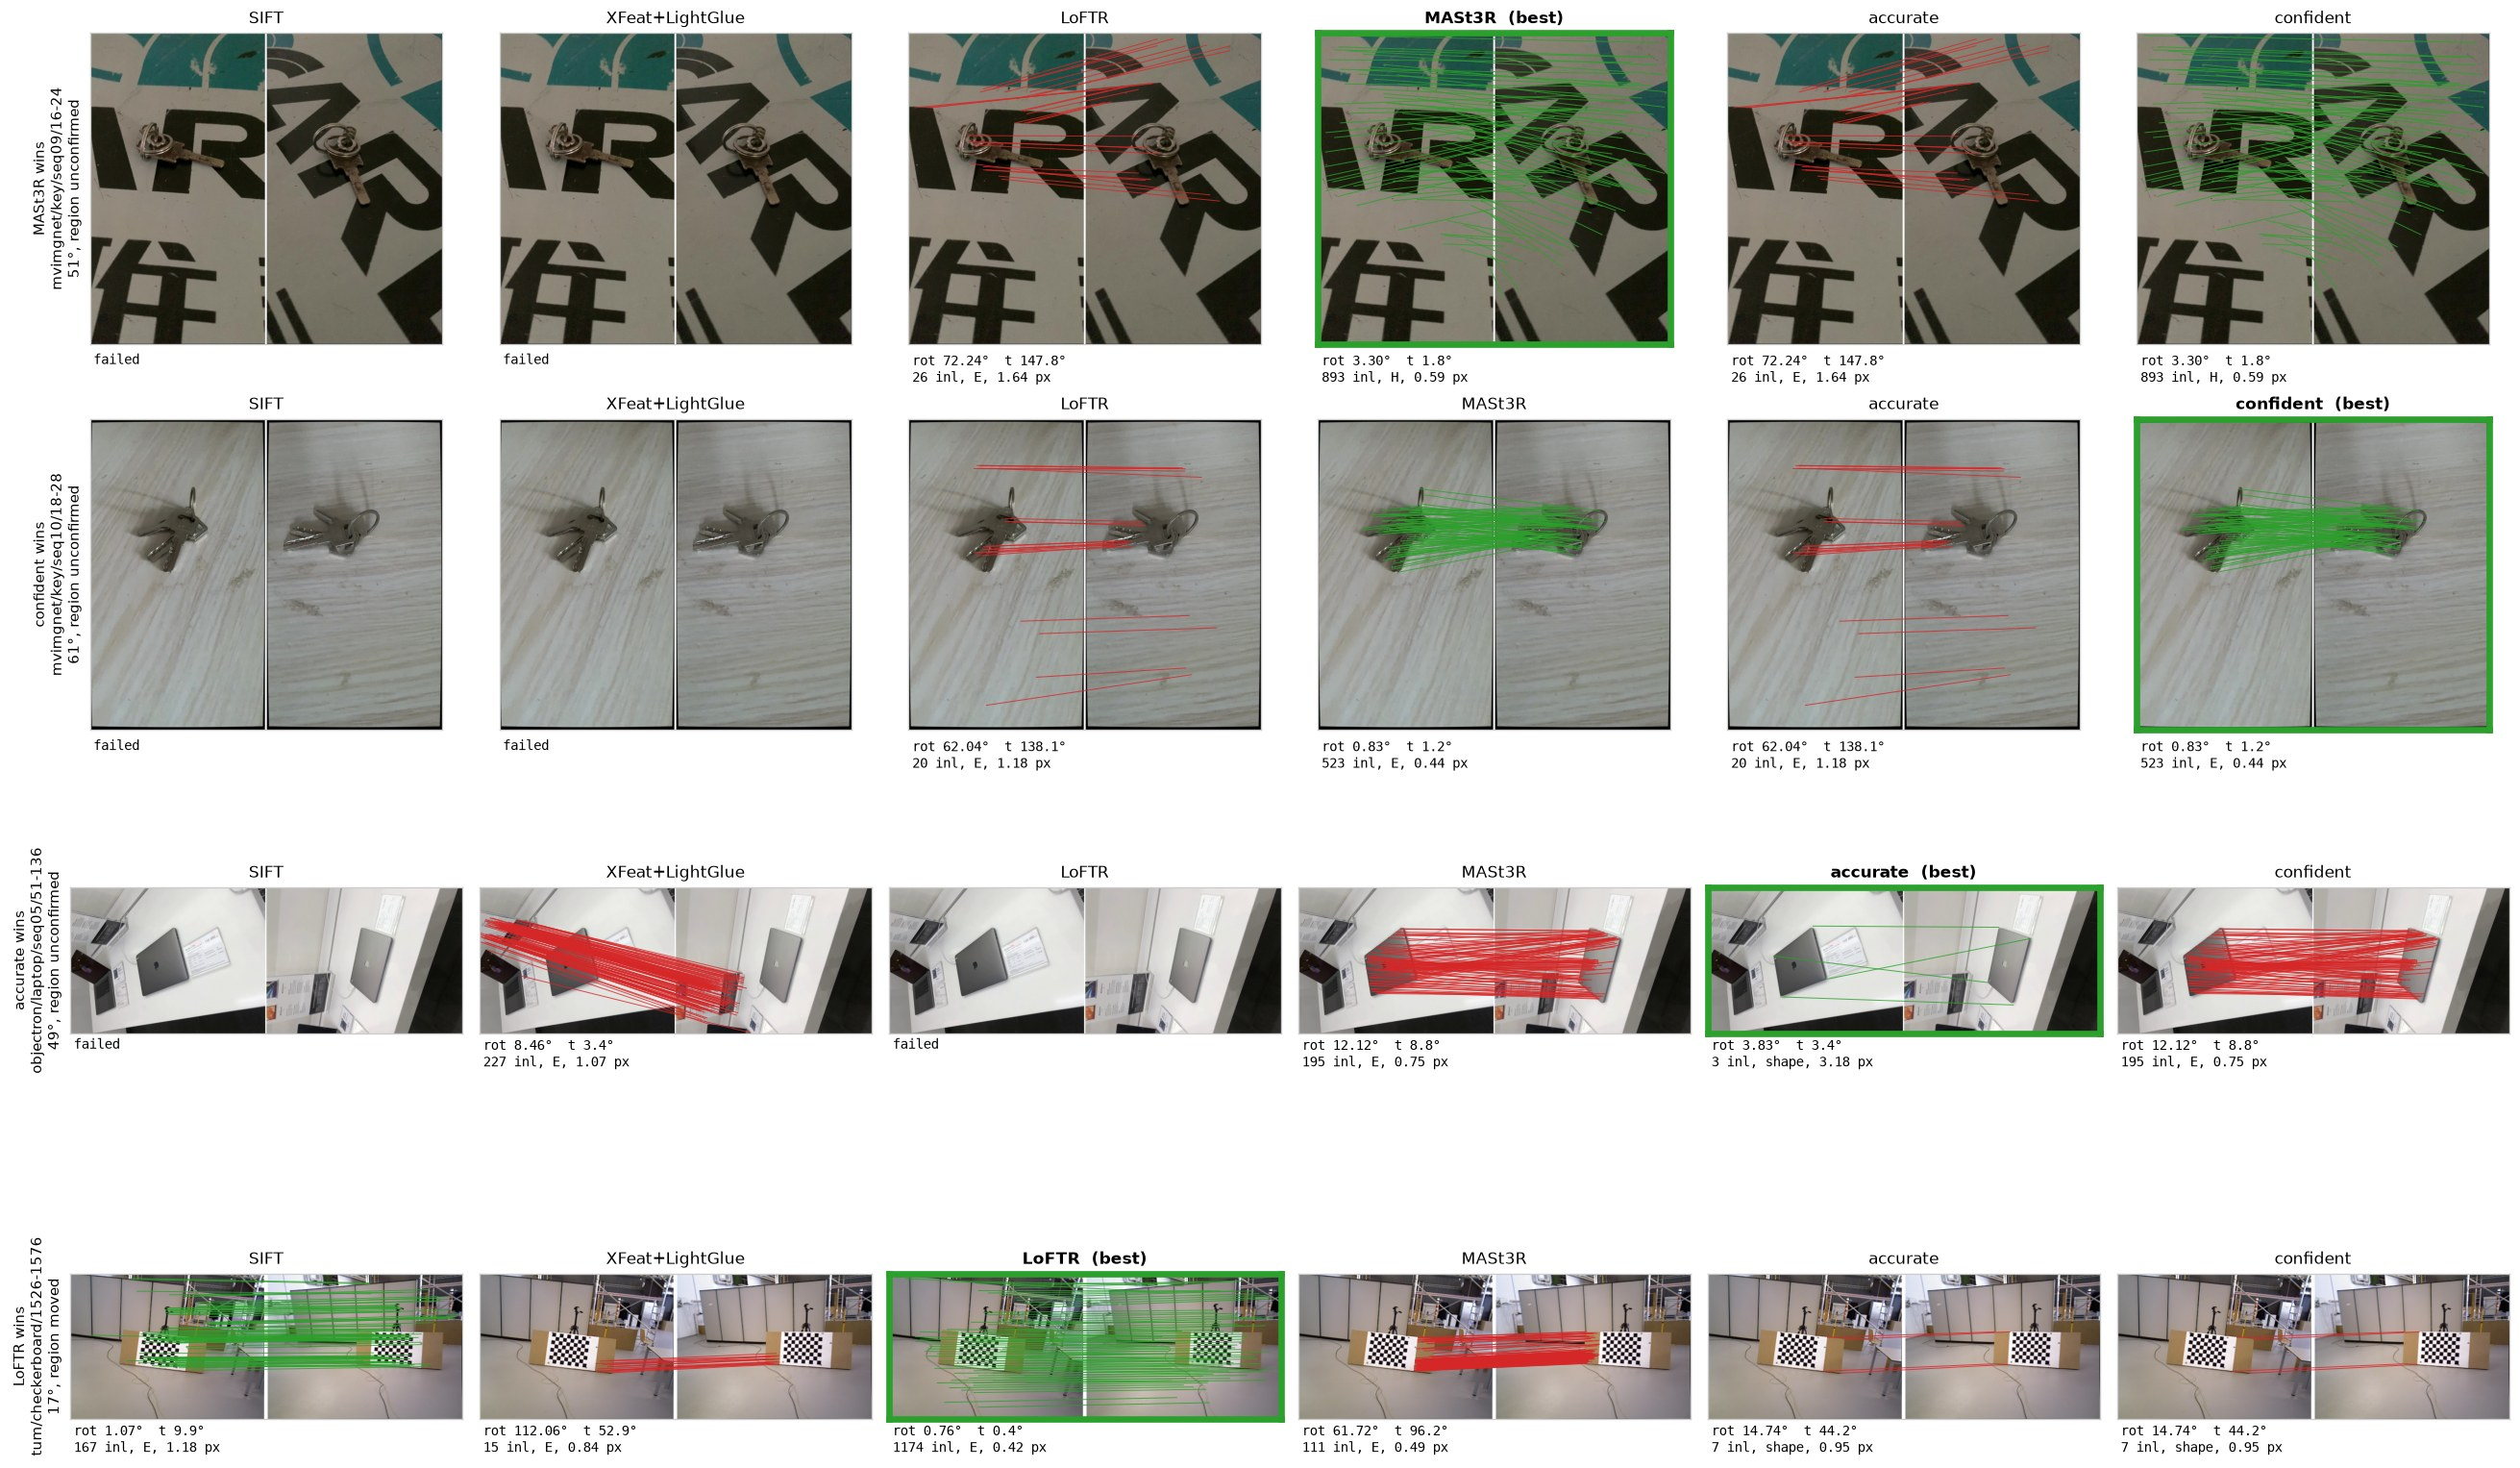
\includegraphics[width=\textwidth]{methods.jpg}
  \caption{Pairs on which one method gives clearly the best pose (framed), with the result of every method, two images only. Inlier correspondences are green when the rotation error is below $5^\circ$ and red otherwise; the text gives the rotation and translation-direction errors, the number of inliers, the selected model and the reprojection error.}
  \label{fig:methods}
\end{figure*}

\subsection{Failure Case}
Figure~\ref{fig:failure} shows the largest remaining error. In a static checkerboard scene the cardboard strip to the right of the board in image~1 is classified as moved and paired with the strip to its left in image~2. Correspondences between the two strips are mutually consistent, and the resulting pose, $61.7^\circ$ in error, has a reprojection error of only 0.49\,px.

\begin{figure*}[t]
  \centering
  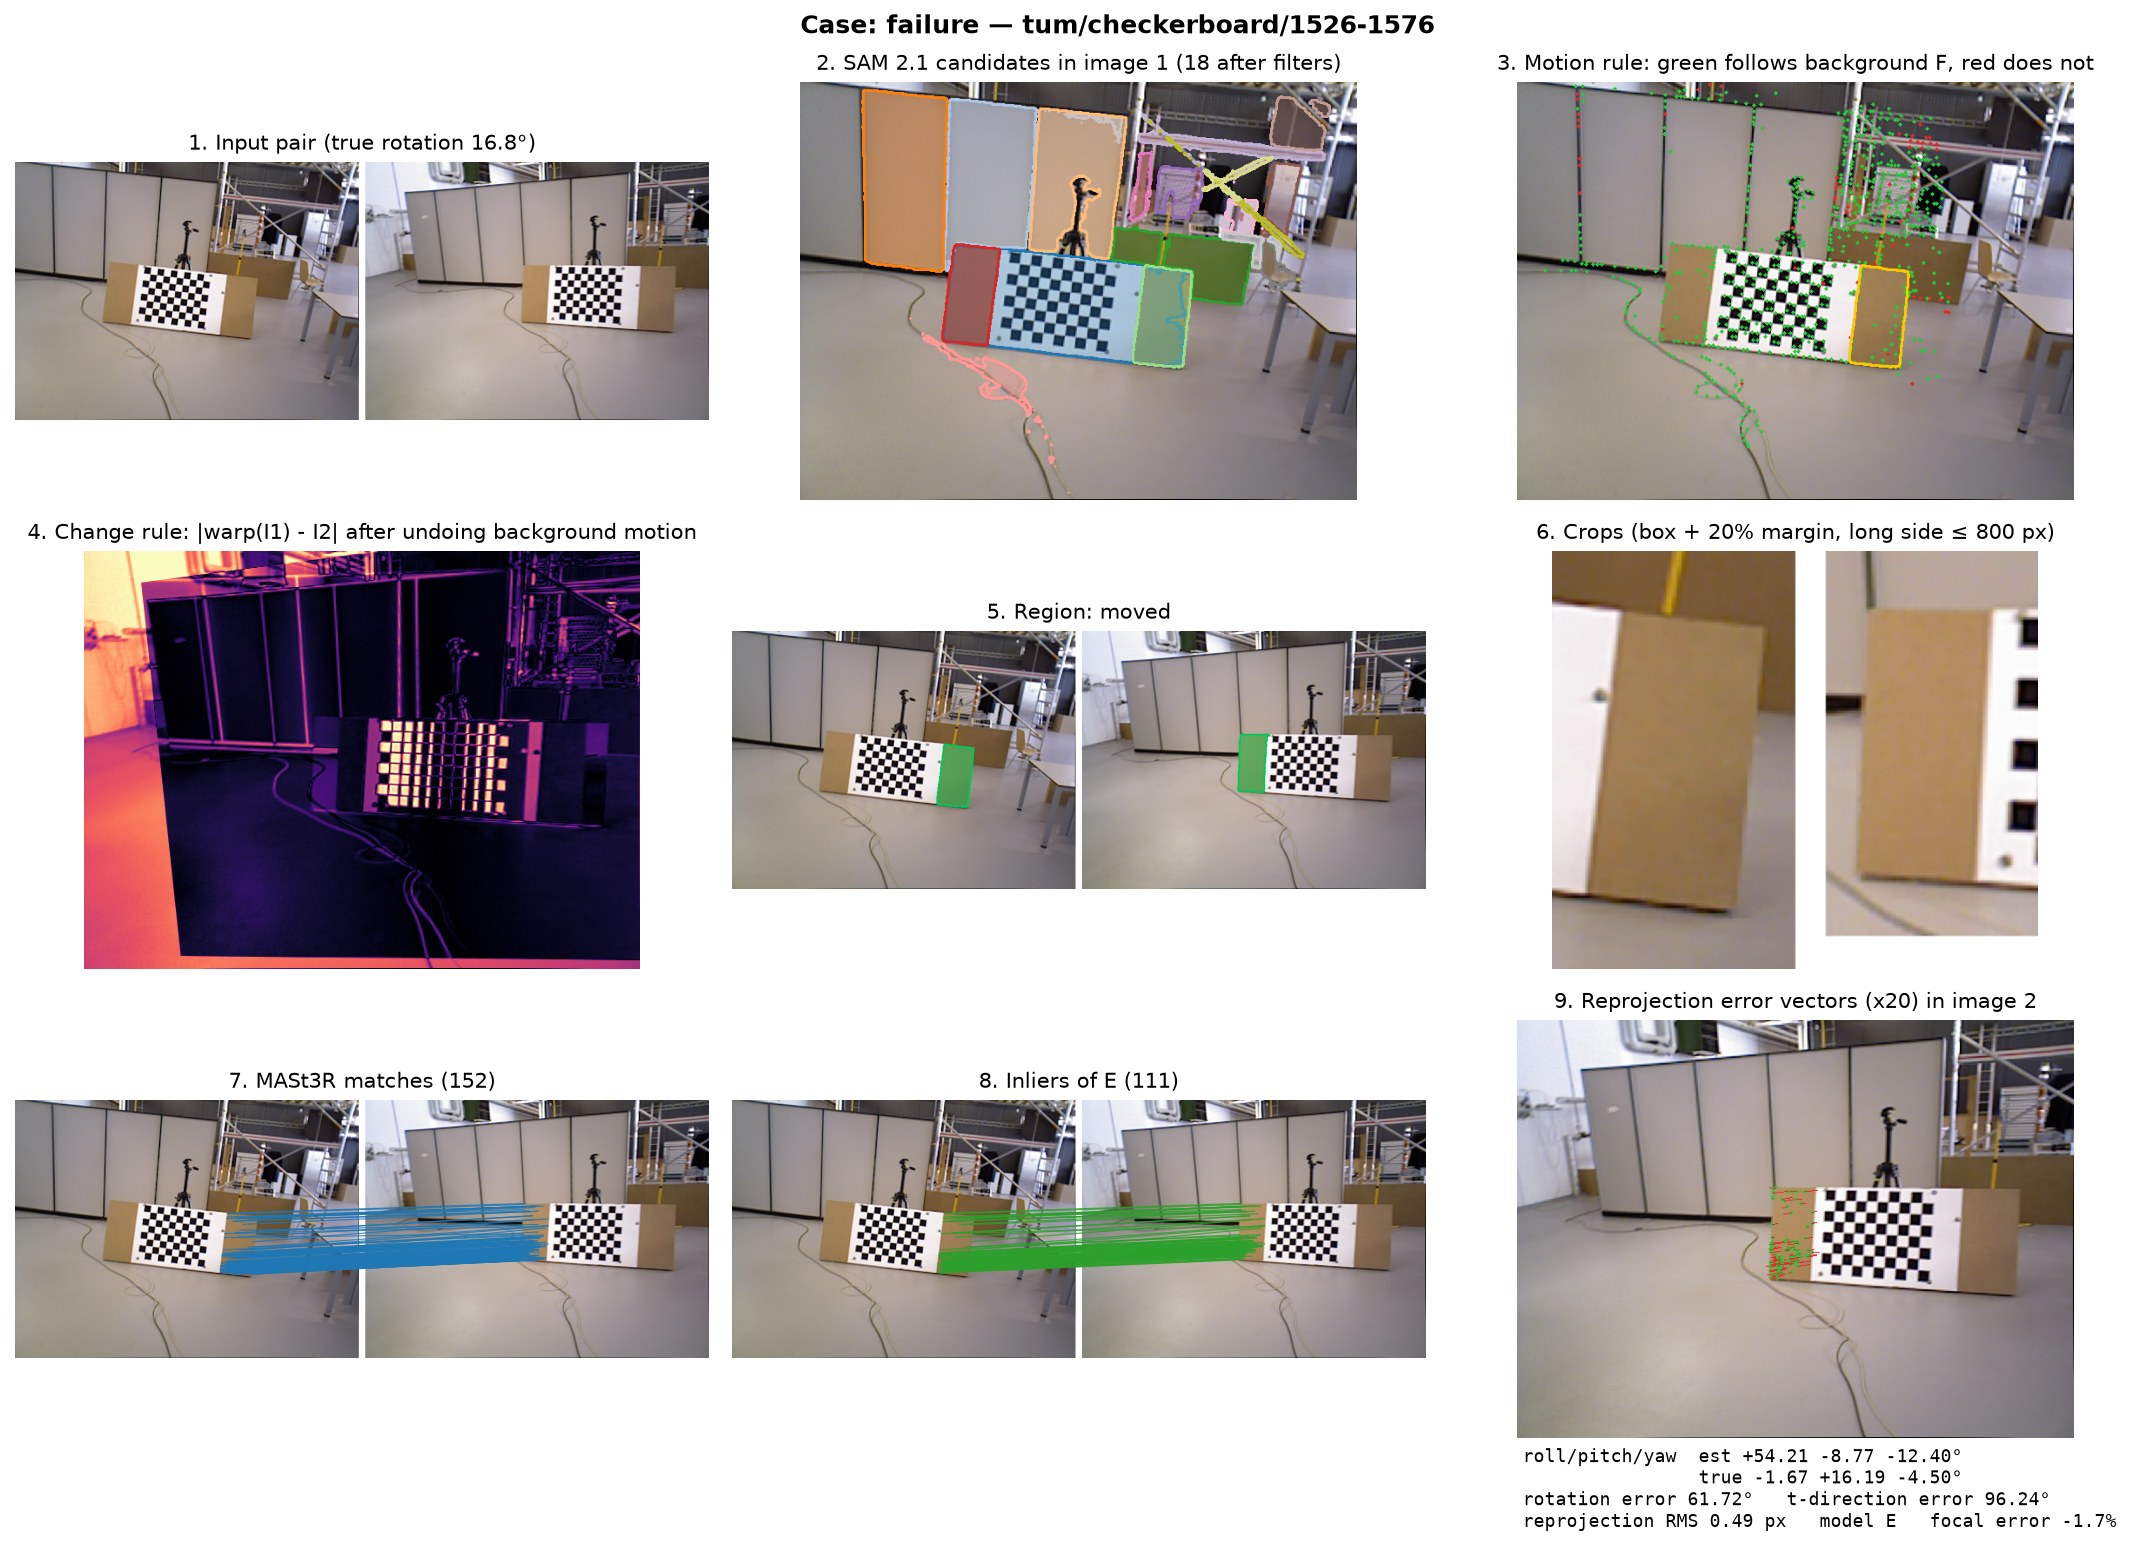
\includegraphics[width=\textwidth]{case_failure.jpg}
  \caption{Failure case (TUM checkerboard, $16.8^\circ$): an incorrect pairing of regions yields a self-consistent but incorrect pose.}
  \label{fig:failure}
\end{figure*}

% ------------------------------------------------------------------ 4
\section{Observations}

\subsection*{4.1 Accuracy of the Two-Image Setting}
\begin{itemize}
  \item \textbf{Estimating the intrinsics and the region costs little.} The pipeline is within one AUC@10 point of the same estimator given the true camera and mask, despite a median focal-length error of 6\%.
  \item \textbf{Rotation is recovered to below one degree} in the typical case (median $0.97^\circ$; per-axis MAE $0.19$--$0.43^\circ$ along a sequence).
  \item \textbf{The translation direction is recovered} whenever the camera moves appreciably (median $0.8$--$1.8^\circ$ from $5^\circ$ upwards), because the essential matrix is used where appropriate and the pose is refined on all inliers.
\end{itemize}

\subsection*{4.2 Matching}
\begin{itemize}
  \item \textbf{MASt3R is the most reliable matcher,} particularly beyond $30^\circ$, where descriptors computed from local appearance change too much.
  \item \textbf{2D matchers remain useful} for textured, moderately rotated objects and are an order of magnitude faster; SIFT's rotation invariance is an advantage for in-plane rotation.
  \item \textbf{The confidence-gated cascade} recovers most of MASt3R's accuracy by sending only doubtful pairs to it.
\end{itemize}

\subsection*{4.3 Reliability Indicators}
\begin{itemize}
  \item \textbf{A low reprojection error does not imply a correct pose}, as the failure case shows.
  \item \textbf{Agreement between independent matchers is informative.} When the rotations from MASt3R and the \texttt{accurate} cascade agree within $2^\circ$ (34 of 56 pairs), no MASt3R rotation error exceeds $10^\circ$; when they disagree, 14\% do.
\end{itemize}

% ------------------------------------------------------------------ 5
\section{Discussion}

\subsection*{5.1 Camera Motion and Object Motion}
The images constrain only relative motion. When the object is moved against a static background, the background's correspondences describe a different motion, which is why the object must be isolated. When nothing moves relative to the background, as in all test sequences used here, the camera's motion relative to the scene equals its motion relative to the object, and using the whole image is correct. The motion and change rules decide between these situations without user input.

\subsection*{5.2 Small and Weakly Textured Objects}
Cropping to the object enlarges it in the matcher's input, and a detector-free, 3D-aware matcher finds correspondences on surfaces where keypoint detectors fail. The remaining difficulty lies in the region decision: a small static patch can resemble a moved object when parallax or blur prevent a local homography from aligning it.

\subsection*{5.3 Observability of Translation}
From two views the translation is determined up to scale, and its direction becomes unobservable as the baseline approaches zero. For consecutive video frames the translation-direction error is large for every method, including with the true intrinsics; this is a property of the geometry rather than of the estimator. The magnitude can be recovered when the object's size is known.

\subsection*{5.4 Planar Ambiguity}
A planar scene admits two poses that explain both images exactly. Choosing between homography and essential matrix by GRIC, breaking the tie with off-plane correspondences, and applying the planar-twin check when the essential matrix is chosen together address this case, which is central to the objects named in the task.

\subsection*{5.5 Limitations}
\begin{itemize}
  \item The region decision can pair incorrect segments in static scenes; the stricter change rule also reduces sensitivity to small, specular objects moved by hand.
  \item The focal-length estimate is less accurate for close-up views with few perspective cues.
  \item MASt3R's descriptors are not rotation-invariant, so large in-plane rotations of flat objects are better handled by SIFT.
  \item Matching with MASt3R takes about 15\,s per pair on a CPU, and the complete pipeline about one minute.
  \item No ground truth was available for coins or plates; the evaluation covers 56 pairs, so per-object figures are indicative.
\end{itemize}

% ------------------------------------------------------------------ 6
\section{Conclusion}
A pipeline was presented that estimates the change in pose of a small object from two RGB images without any additional input. The focal length is obtained from a predicted point map, the moved object is identified by geometric and photometric consistency with the background, and the pose is computed from 3D-aware correspondences with a planar/non-planar model choice, an explicit treatment of the planar ambiguity and non-linear refinement. On 56 held-out pairs from four datasets, the median rotation error is $0.97^\circ$, the median translation-direction error $1.79^\circ$ and the median reprojection error 0.46\,px, within one point of AUC@10 of the same estimator given the true camera and object mask; along a TUM sequence the per-axis rotation errors are below $0.5^\circ$. The principal remaining errors arise from the region decision in static scenes and from the unobservability of translation over very short baselines. Future work includes enforcing agreement between independent matchers in the verdict and tracking the object region jointly across both images.

\section*{Data availability}
The code and results are available at\\ \url{https://github.com/Svanik277373/CS6350_Pose_Estimation_Project}.

\begin{thebibliography}{99}\small
\bibitem{hz} R.~Hartley and A.~Zisserman, \emph{Multiple View Geometry in Computer Vision}, 2nd ed. Cambridge University Press, 2004.
\bibitem{longuethiggins} H.~C. Longuet-Higgins, ``A computer algorithm for reconstructing a scene from two projections,'' \emph{Nature}, vol.~293, pp.~133--135, 1981.
\bibitem{nister} D.~Nist\'er, ``An efficient solution to the five-point relative pose problem,'' \emph{IEEE Trans.\ PAMI}, vol.~26, no.~6, pp.~756--770, 2004.
\bibitem{faugeras} O.~Faugeras and F.~Lustman, ``Motion and structure from motion in a piecewise planar environment,'' \emph{Int.\ J.\ Pattern Recognition and Artificial Intelligence}, vol.~2, no.~3, pp.~485--508, 1988.
\bibitem{malis} E.~Malis and M.~Vargas, ``Deeper understanding of the homography decomposition for vision-based control,'' INRIA, Tech.\ Rep.\ RR-6303, 2007.
\bibitem{torr} P.~H.~S. Torr, ``Geometric motion segmentation and model selection,'' \emph{Phil.\ Trans.\ Royal Society A}, vol.~356, pp.~1321--1340, 1998.
\bibitem{ransac} M.~A. Fischler and R.~C. Bolles, ``Random sample consensus,'' \emph{Communications of the ACM}, vol.~24, no.~6, pp.~381--395, 1981.
\bibitem{magsac} D.~Barath, J.~Noskova, M.~Ivashechkin and J.~Matas, ``MAGSAC++, a fast, reliable and accurate robust estimator,'' in \emph{CVPR}, 2020.
\bibitem{sift} D.~G. Lowe, ``Distinctive image features from scale-invariant keypoints,'' \emph{IJCV}, vol.~60, no.~2, pp.~91--110, 2004.
\bibitem{xfeat} G.~Potje, F.~Cadar, A.~Araujo, R.~Martins and E.~R. Nascimento, ``XFeat: Accelerated features for lightweight image matching,'' in \emph{CVPR}, 2024.
\bibitem{lightglue} P.~Lindenberger, P.-E. Sarlin and M.~Pollefeys, ``LightGlue: Local feature matching at light speed,'' in \emph{ICCV}, 2023.
\bibitem{superglue} P.-E. Sarlin, D.~DeTone, T.~Malisiewicz and A.~Rabinovich, ``SuperGlue: Learning feature matching with graph neural networks,'' in \emph{CVPR}, 2020.
\bibitem{loftr} J.~Sun, Z.~Shen, Y.~Wang, H.~Bao and X.~Zhou, ``LoFTR: Detector-free local feature matching with transformers,'' in \emph{CVPR}, 2021.
\bibitem{dust3r} S.~Wang, V.~Leroy, Y.~Cabon, B.~Chidlovskii and J.~Revaud, ``DUSt3R: Geometric 3D vision made easy,'' in \emph{CVPR}, 2024.
\bibitem{mast3r} V.~Leroy, Y.~Cabon and J.~Revaud, ``Grounding image matching in 3D with MASt3R,'' in \emph{ECCV}, 2024.
\bibitem{sam} A.~Kirillov \emph{et al.}, ``Segment anything,'' in \emph{ICCV}, 2023.
\bibitem{sam2} N.~Ravi \emph{et al.}, ``SAM 2: Segment anything in images and videos,'' arXiv:2408.00714, 2024.
\bibitem{hiera} C.~Ryali \emph{et al.}, ``Hiera: A hierarchical vision transformer without the bells-and-whistles,'' in \emph{ICML}, 2023.
\bibitem{irani} M.~Irani and P.~Anandan, ``A unified approach to moving object detection in 2D and 3D scenes,'' \emph{IEEE Trans.\ PAMI}, vol.~20, no.~6, pp.~577--589, 1998.
\bibitem{lewis} J.~P. Lewis, ``Fast normalized cross-correlation,'' in \emph{Vision Interface}, 1995.
\bibitem{weiszfeld} E.~Weiszfeld, ``Sur le point pour lequel la somme des distances de $n$ points donn\'es est minimum,'' \emph{T\^ohoku Mathematical Journal}, vol.~43, pp.~355--386, 1937.
\bibitem{levenberg} K.~Levenberg, ``A method for the solution of certain non-linear problems in least squares,'' \emph{Quarterly of Applied Mathematics}, vol.~2, pp.~164--168, 1944.
\bibitem{marquardt} D.~W. Marquardt, ``An algorithm for least-squares estimation of nonlinear parameters,'' \emph{SIAM J.\ Applied Mathematics}, vol.~11, no.~2, pp.~431--441, 1963.
\bibitem{tum} J.~Sturm, N.~Engelhard, F.~Endres, W.~Burgard and D.~Cremers, ``A benchmark for the evaluation of RGB-D SLAM systems,'' in \emph{IROS}, 2012.
\bibitem{objectron} A.~Ahmadyan, L.~Zhang, A.~Ablavatski, J.~Wei and M.~Grundmann, ``Objectron: A large scale dataset of object-centric videos in the wild with pose annotations,'' in \emph{CVPR}, 2021.
\bibitem{co3d} J.~Reizenstein \emph{et al.}, ``Common Objects in 3D: Large-scale learning and evaluation of real-life 3D category reconstruction,'' in \emph{ICCV}, 2021.
\bibitem{mvimgnet} X.~Yu \emph{et al.}, ``MVImgNet: A large-scale dataset of multi-view images,'' in \emph{CVPR}, 2023.
\bibitem{zhang} Z.~Zhang, ``A flexible new technique for camera calibration,'' \emph{IEEE Trans.\ PAMI}, vol.~22, no.~11, pp.~1330--1334, 2000.
\end{thebibliography}

% ------------------------------------------------------------------ 7
\section{Supplementary Data}

This section reports qualitative outputs for further cases and a component study in which the dataset intrinsics and object regions are supplied, isolating the effect of each part of the pose estimator.

\subsection{Qualitative Pipeline Outputs}
Figures~\ref{fig:case-3d}--\ref{fig:case-tiny} show the stages of the pipeline for a three-dimensional object, a small object, a large viewpoint change and consecutive frames.

\begin{figure*}[p]
  \centering
  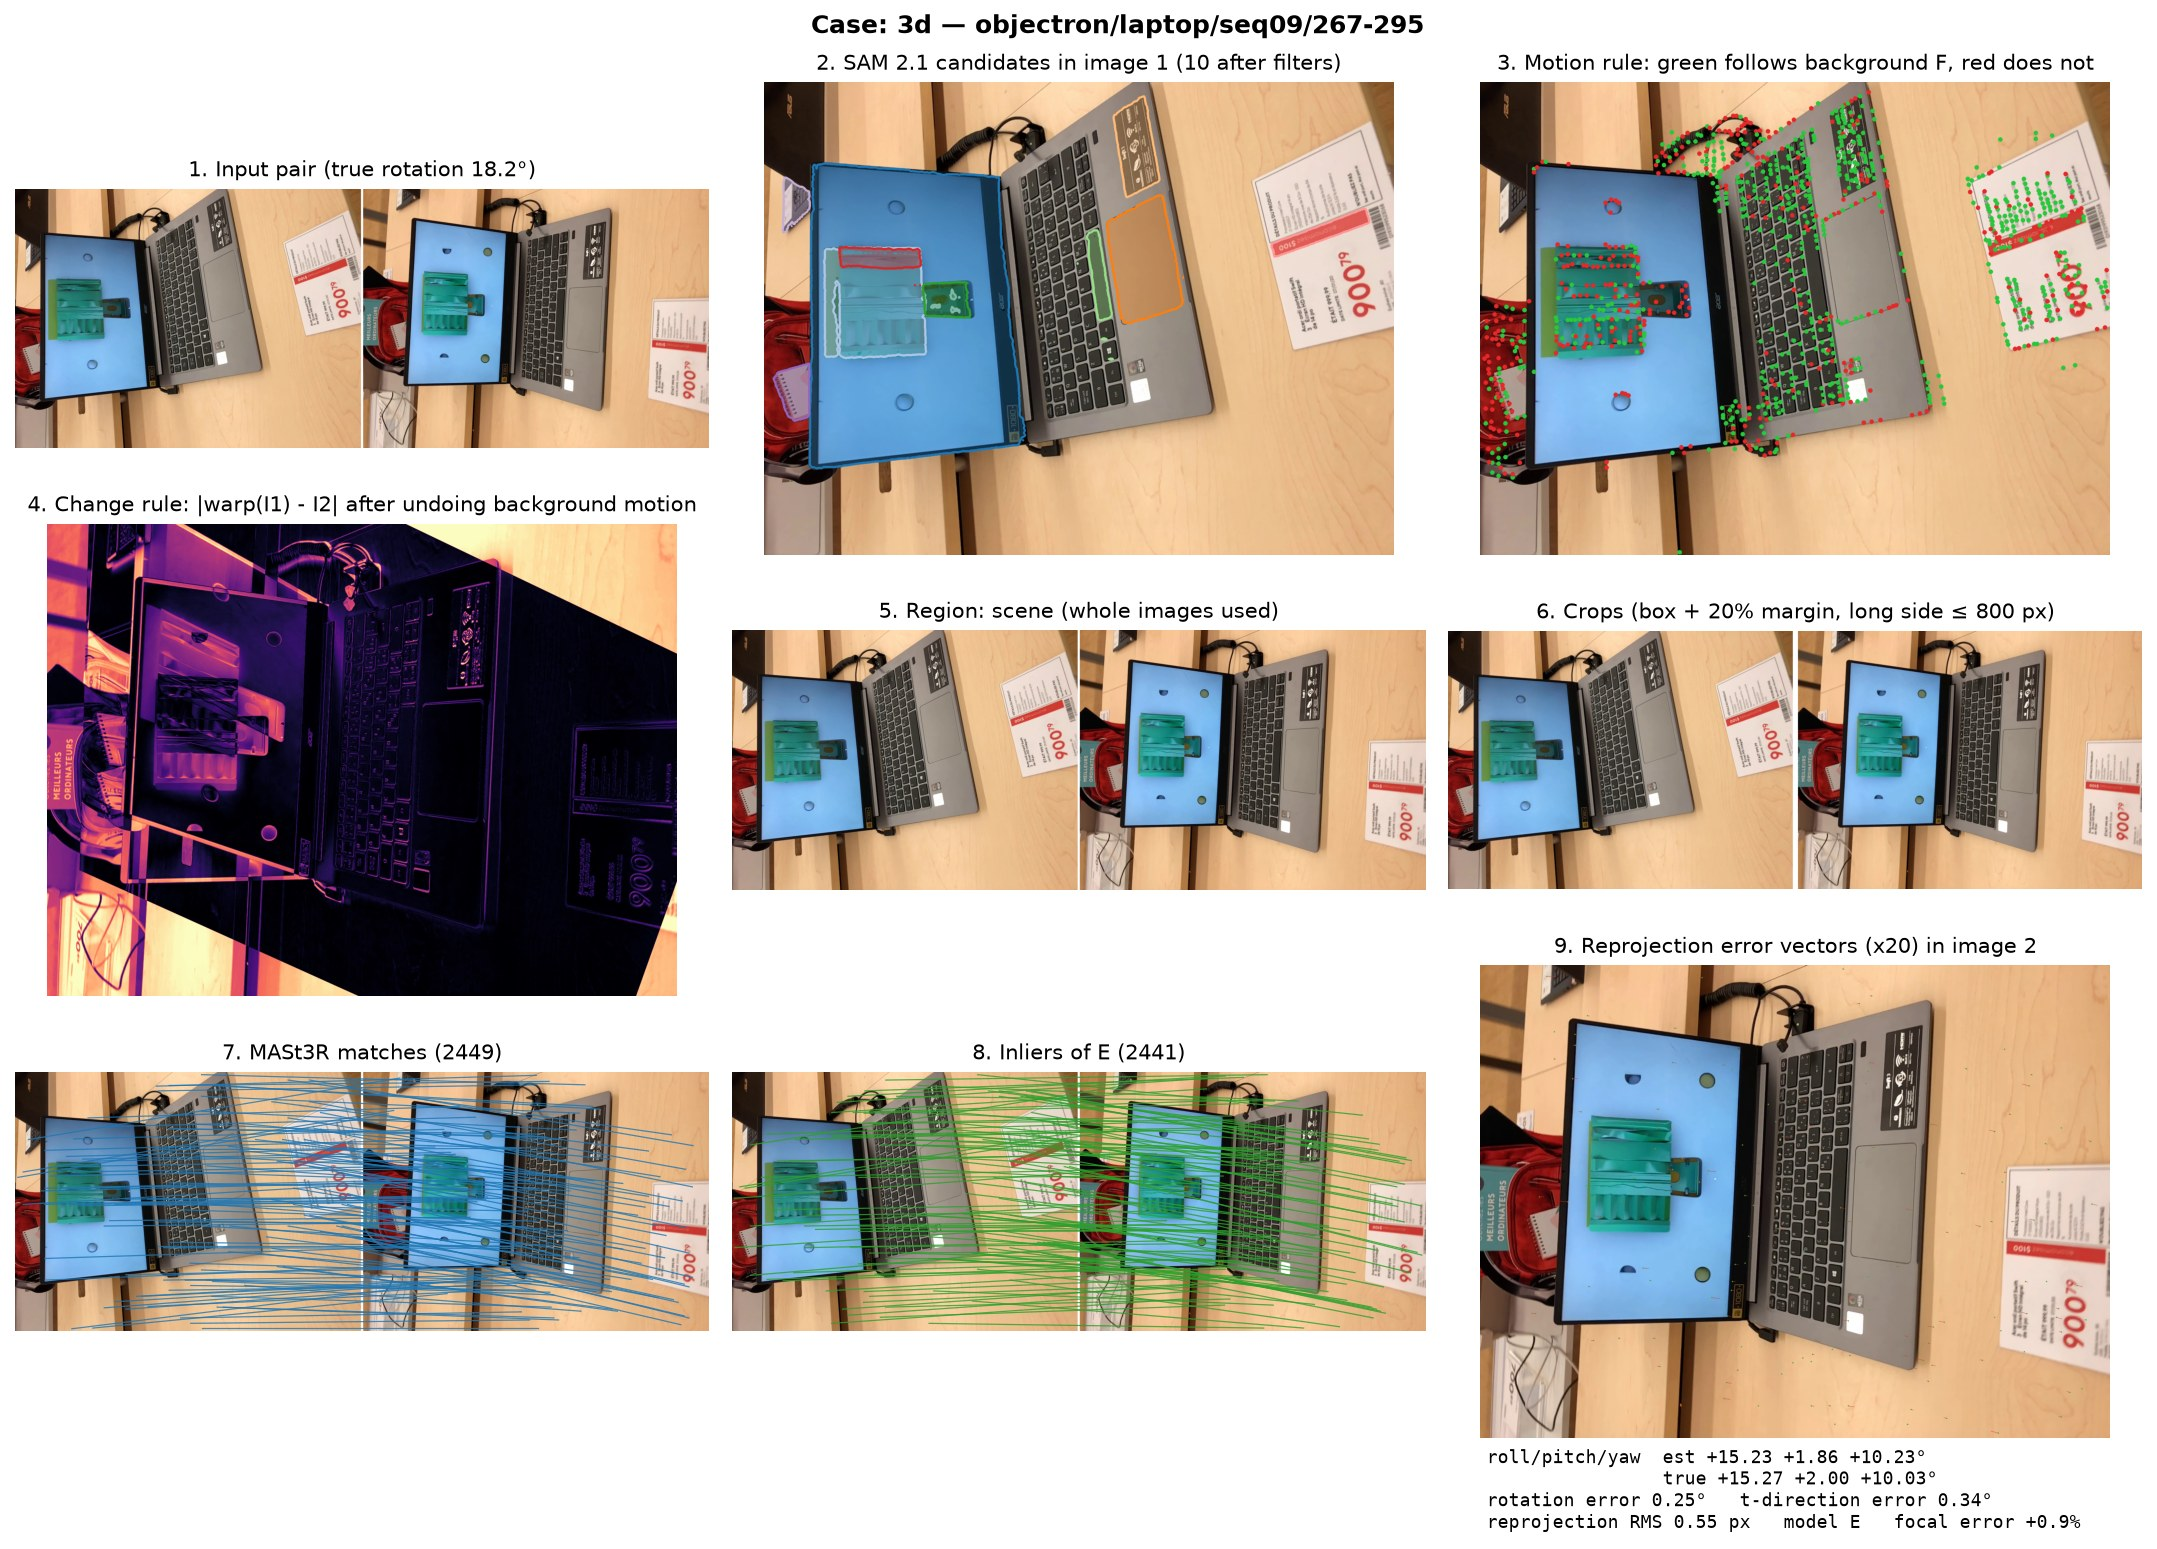
\includegraphics[width=\textwidth]{case_3d.jpg}
  \caption{Three-dimensional object (Objectron laptop, $18.2^\circ$): rotation error $0.25^\circ$.}
  \label{fig:case-3d}
\end{figure*}
\begin{figure*}[p]
  \centering
  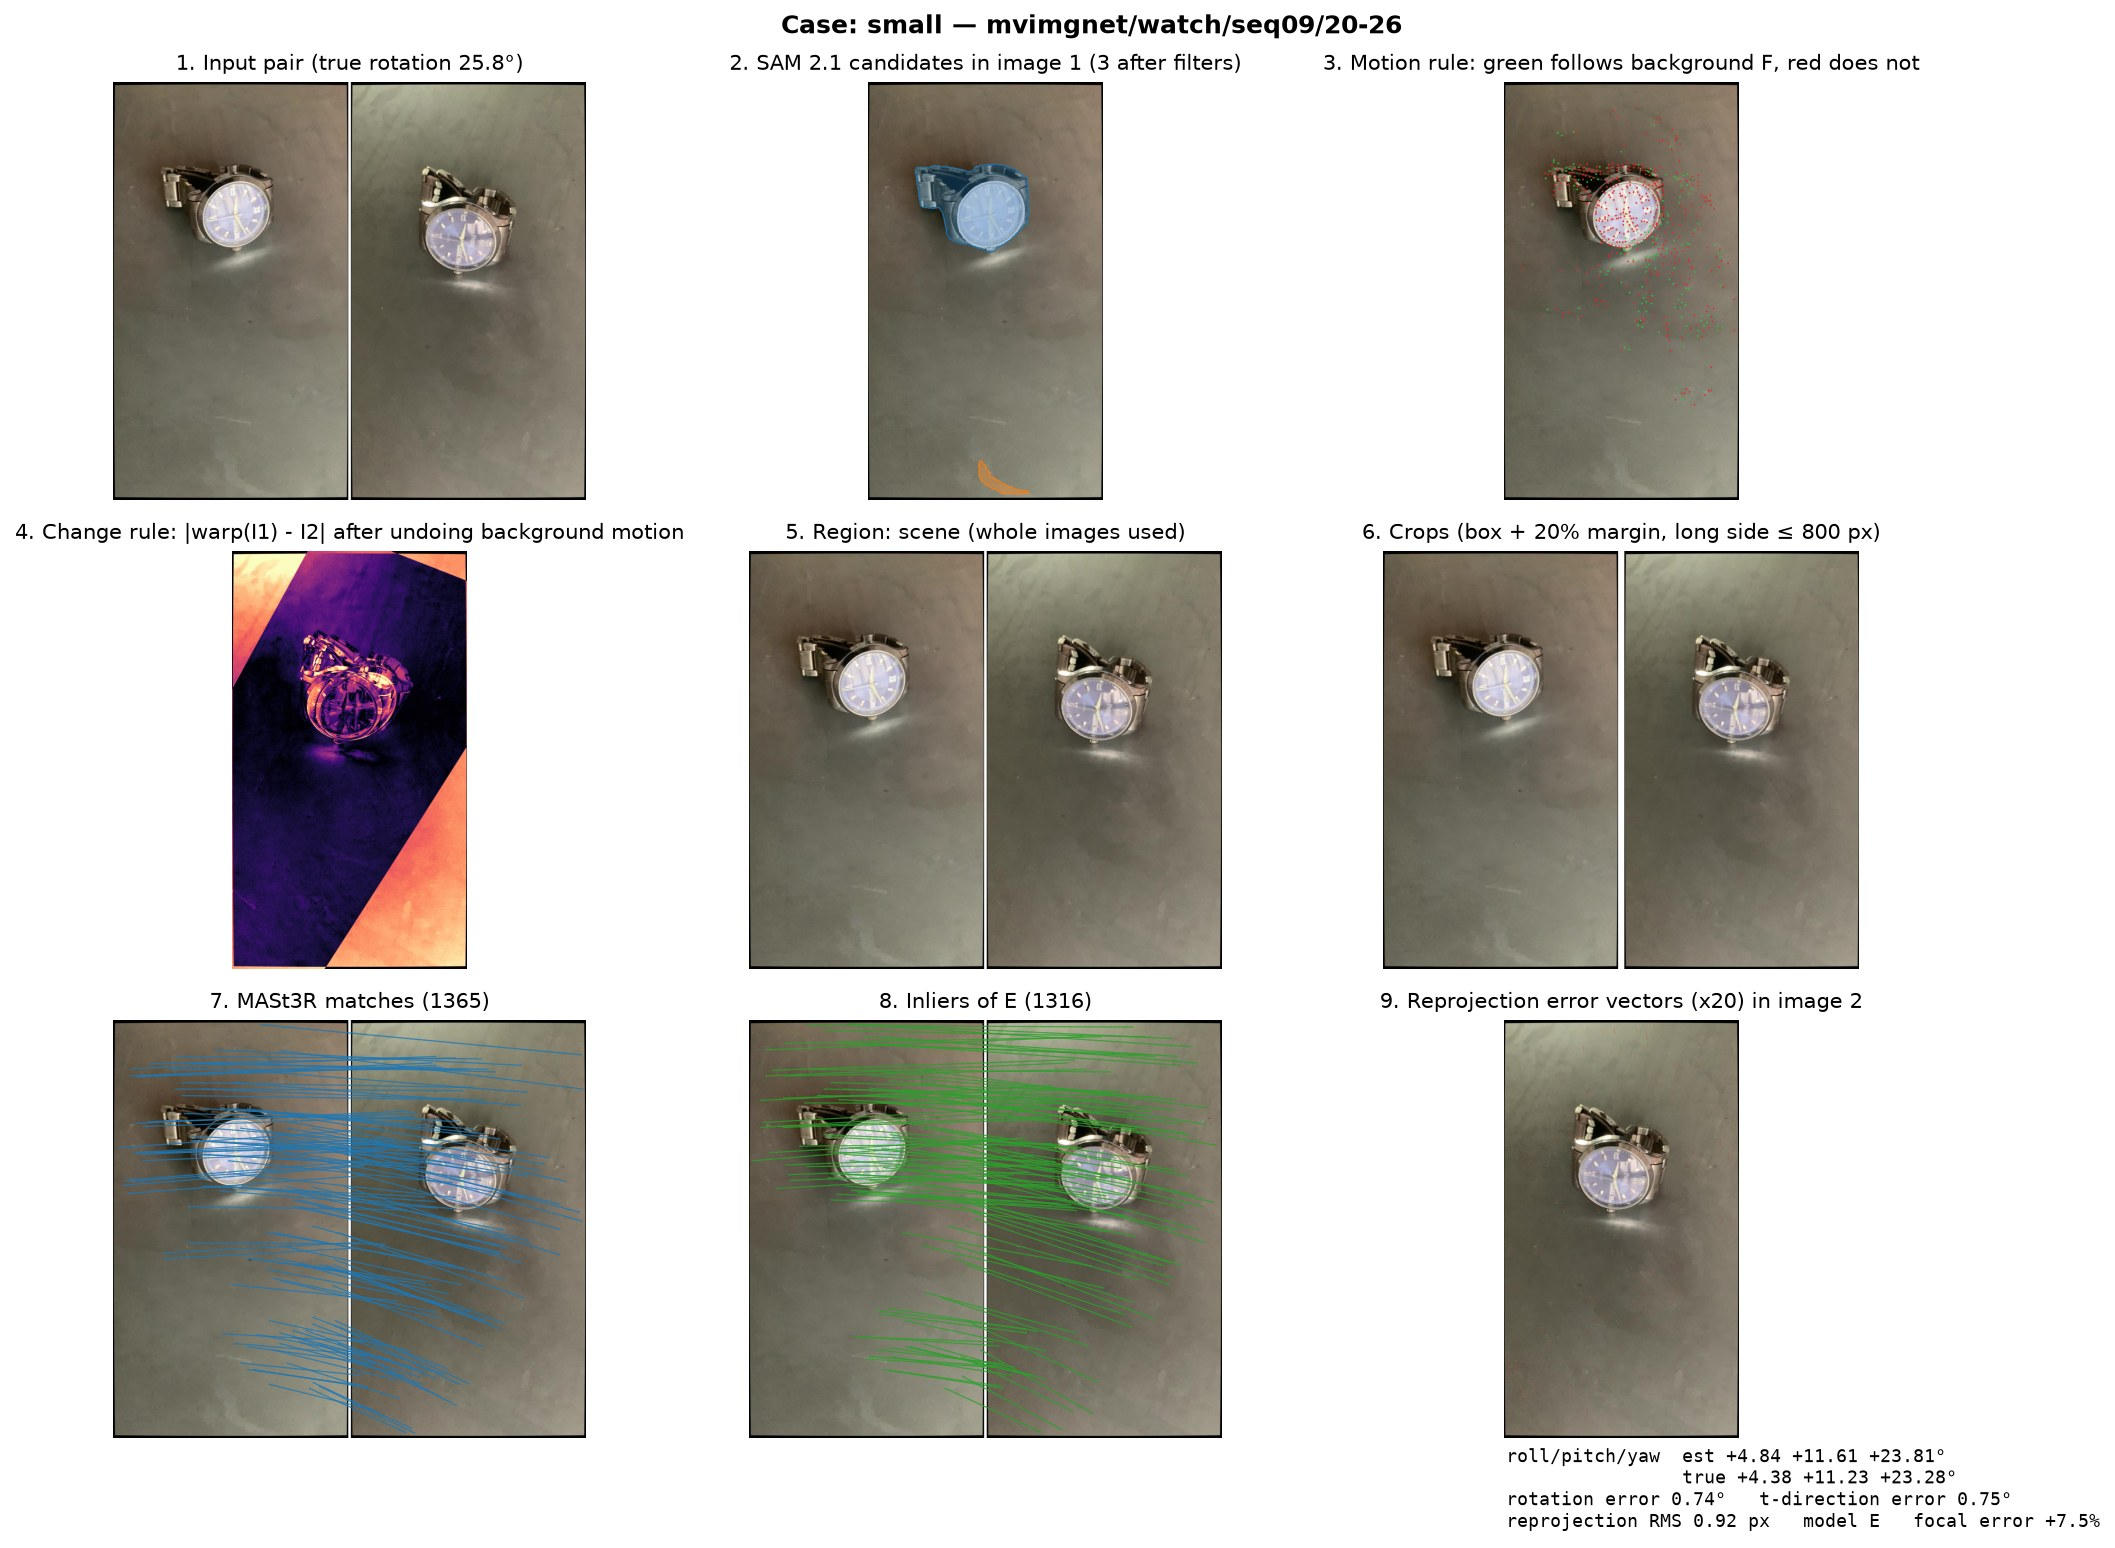
\includegraphics[width=\textwidth]{case_small.jpg}
  \caption{Small object (MVImgNet watch, $25.8^\circ$): rotation error $0.74^\circ$.}
  \label{fig:case-small}
\end{figure*}
\begin{figure*}[p]
  \centering
  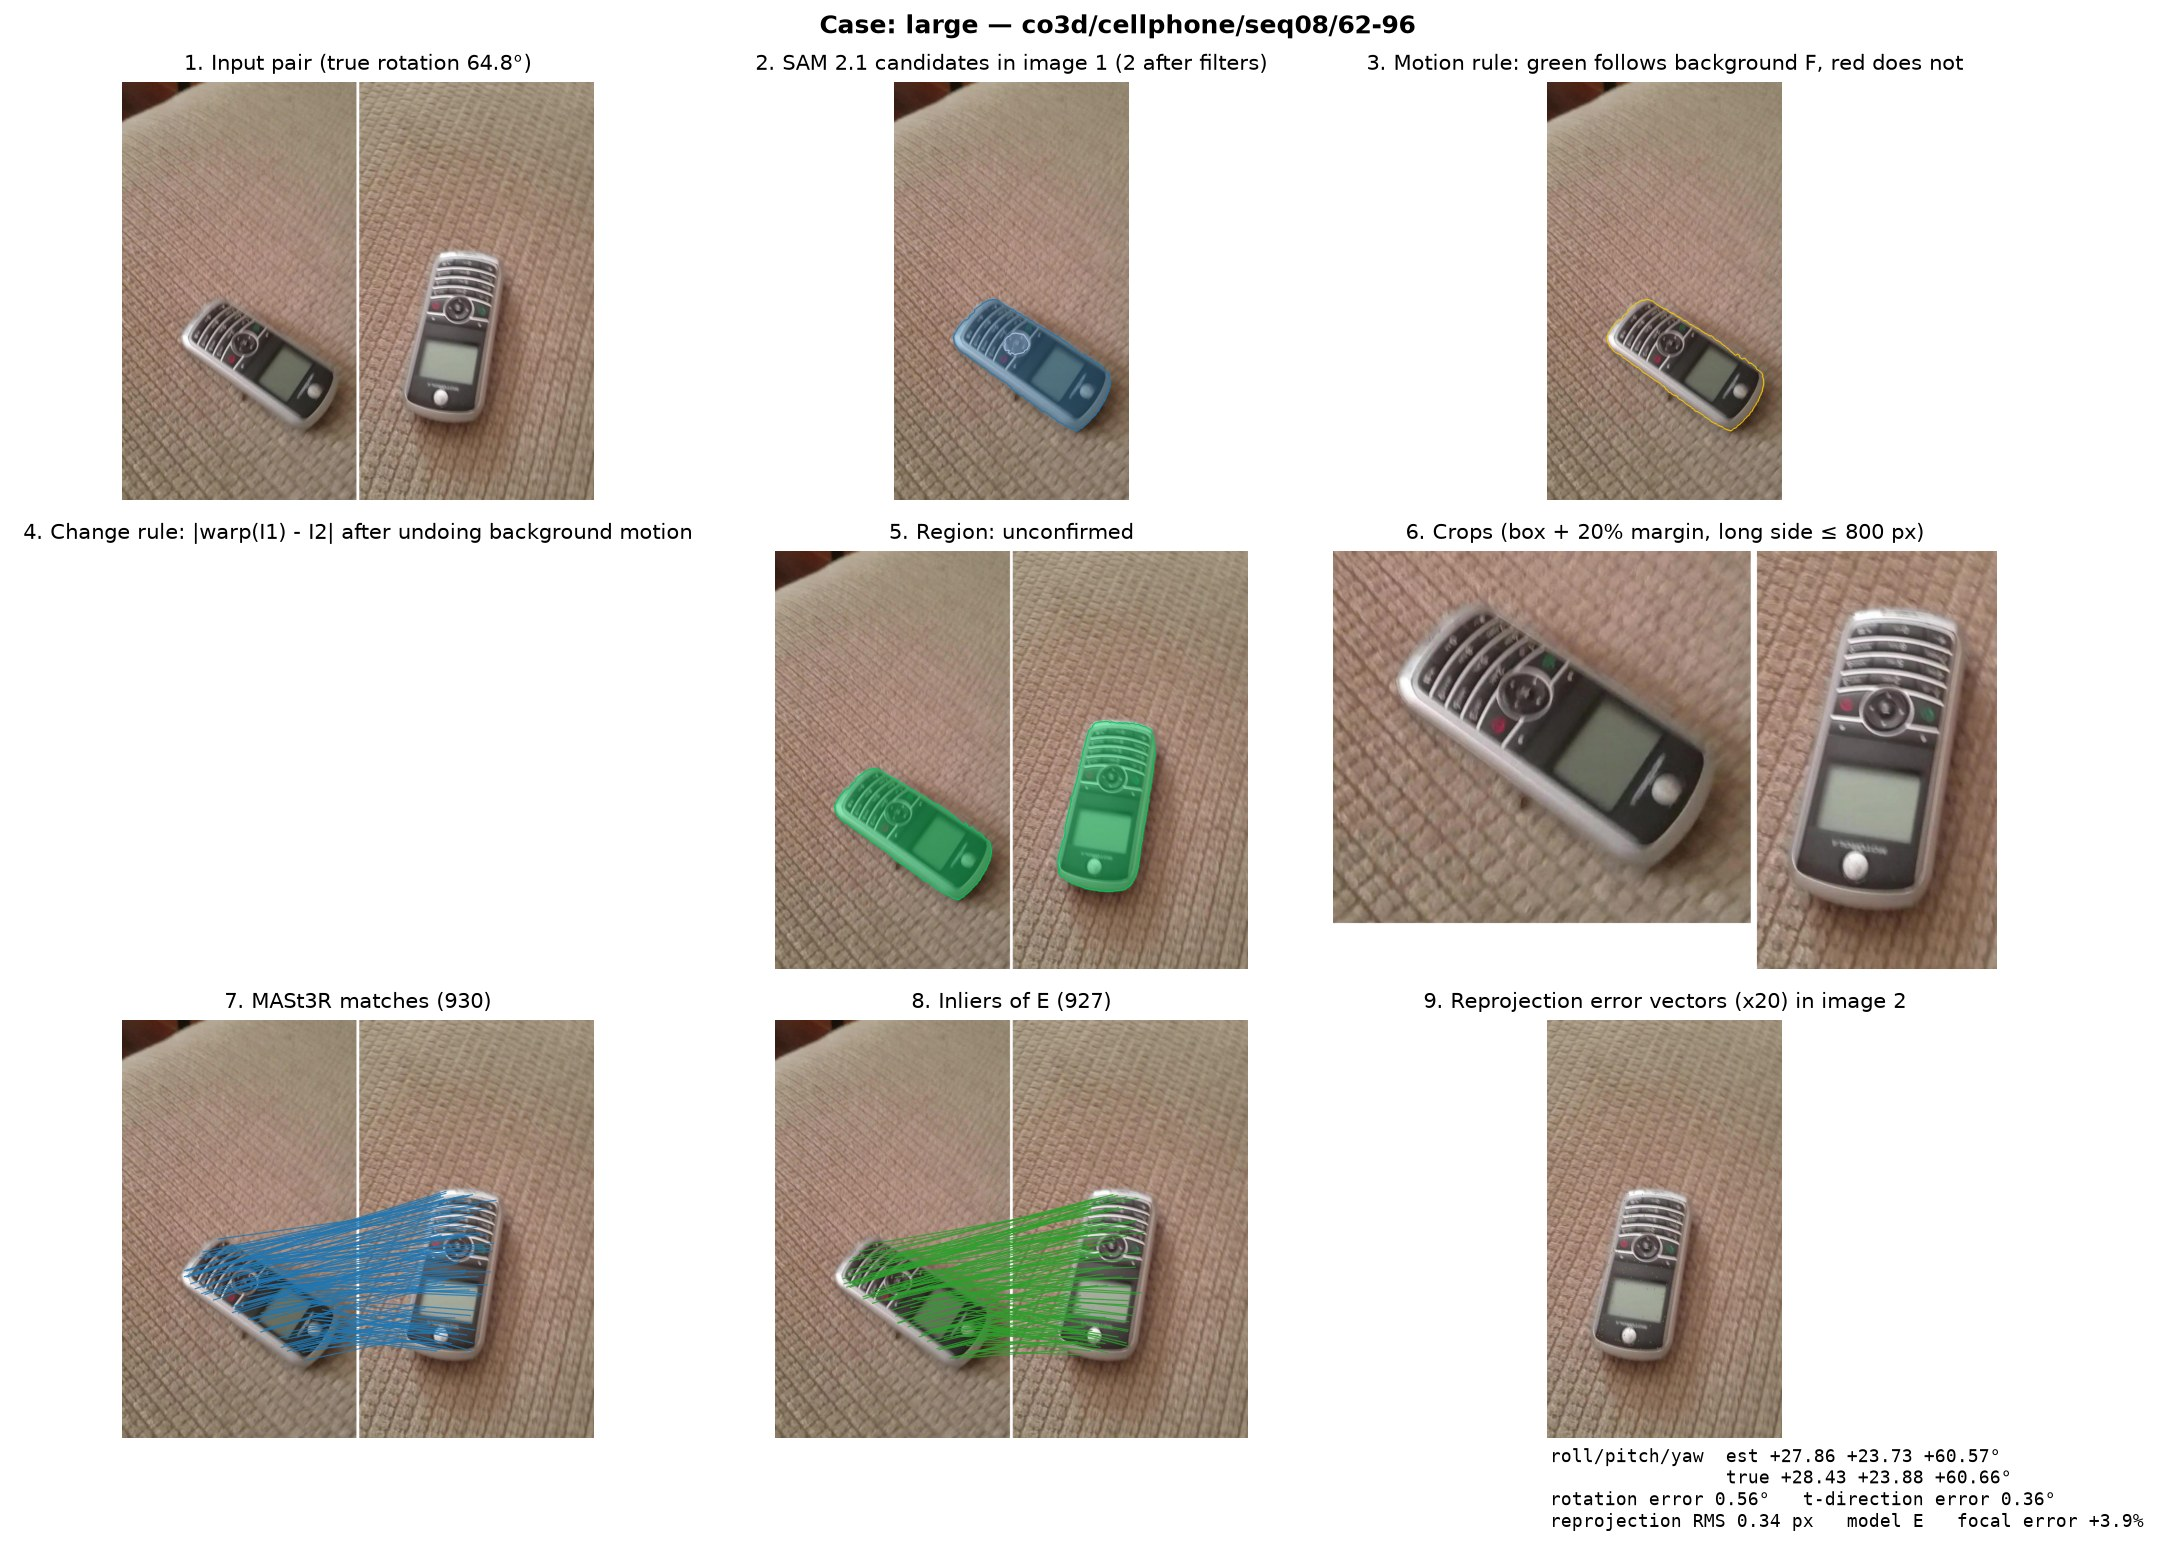
\includegraphics[width=\textwidth]{case_large.jpg}
  \caption{Large viewpoint change (CO3D mobile phone, $64.8^\circ$): region unconfirmed, rotation error $0.56^\circ$.}
  \label{fig:case-large}
\end{figure*}
\begin{figure*}[p]
  \centering
  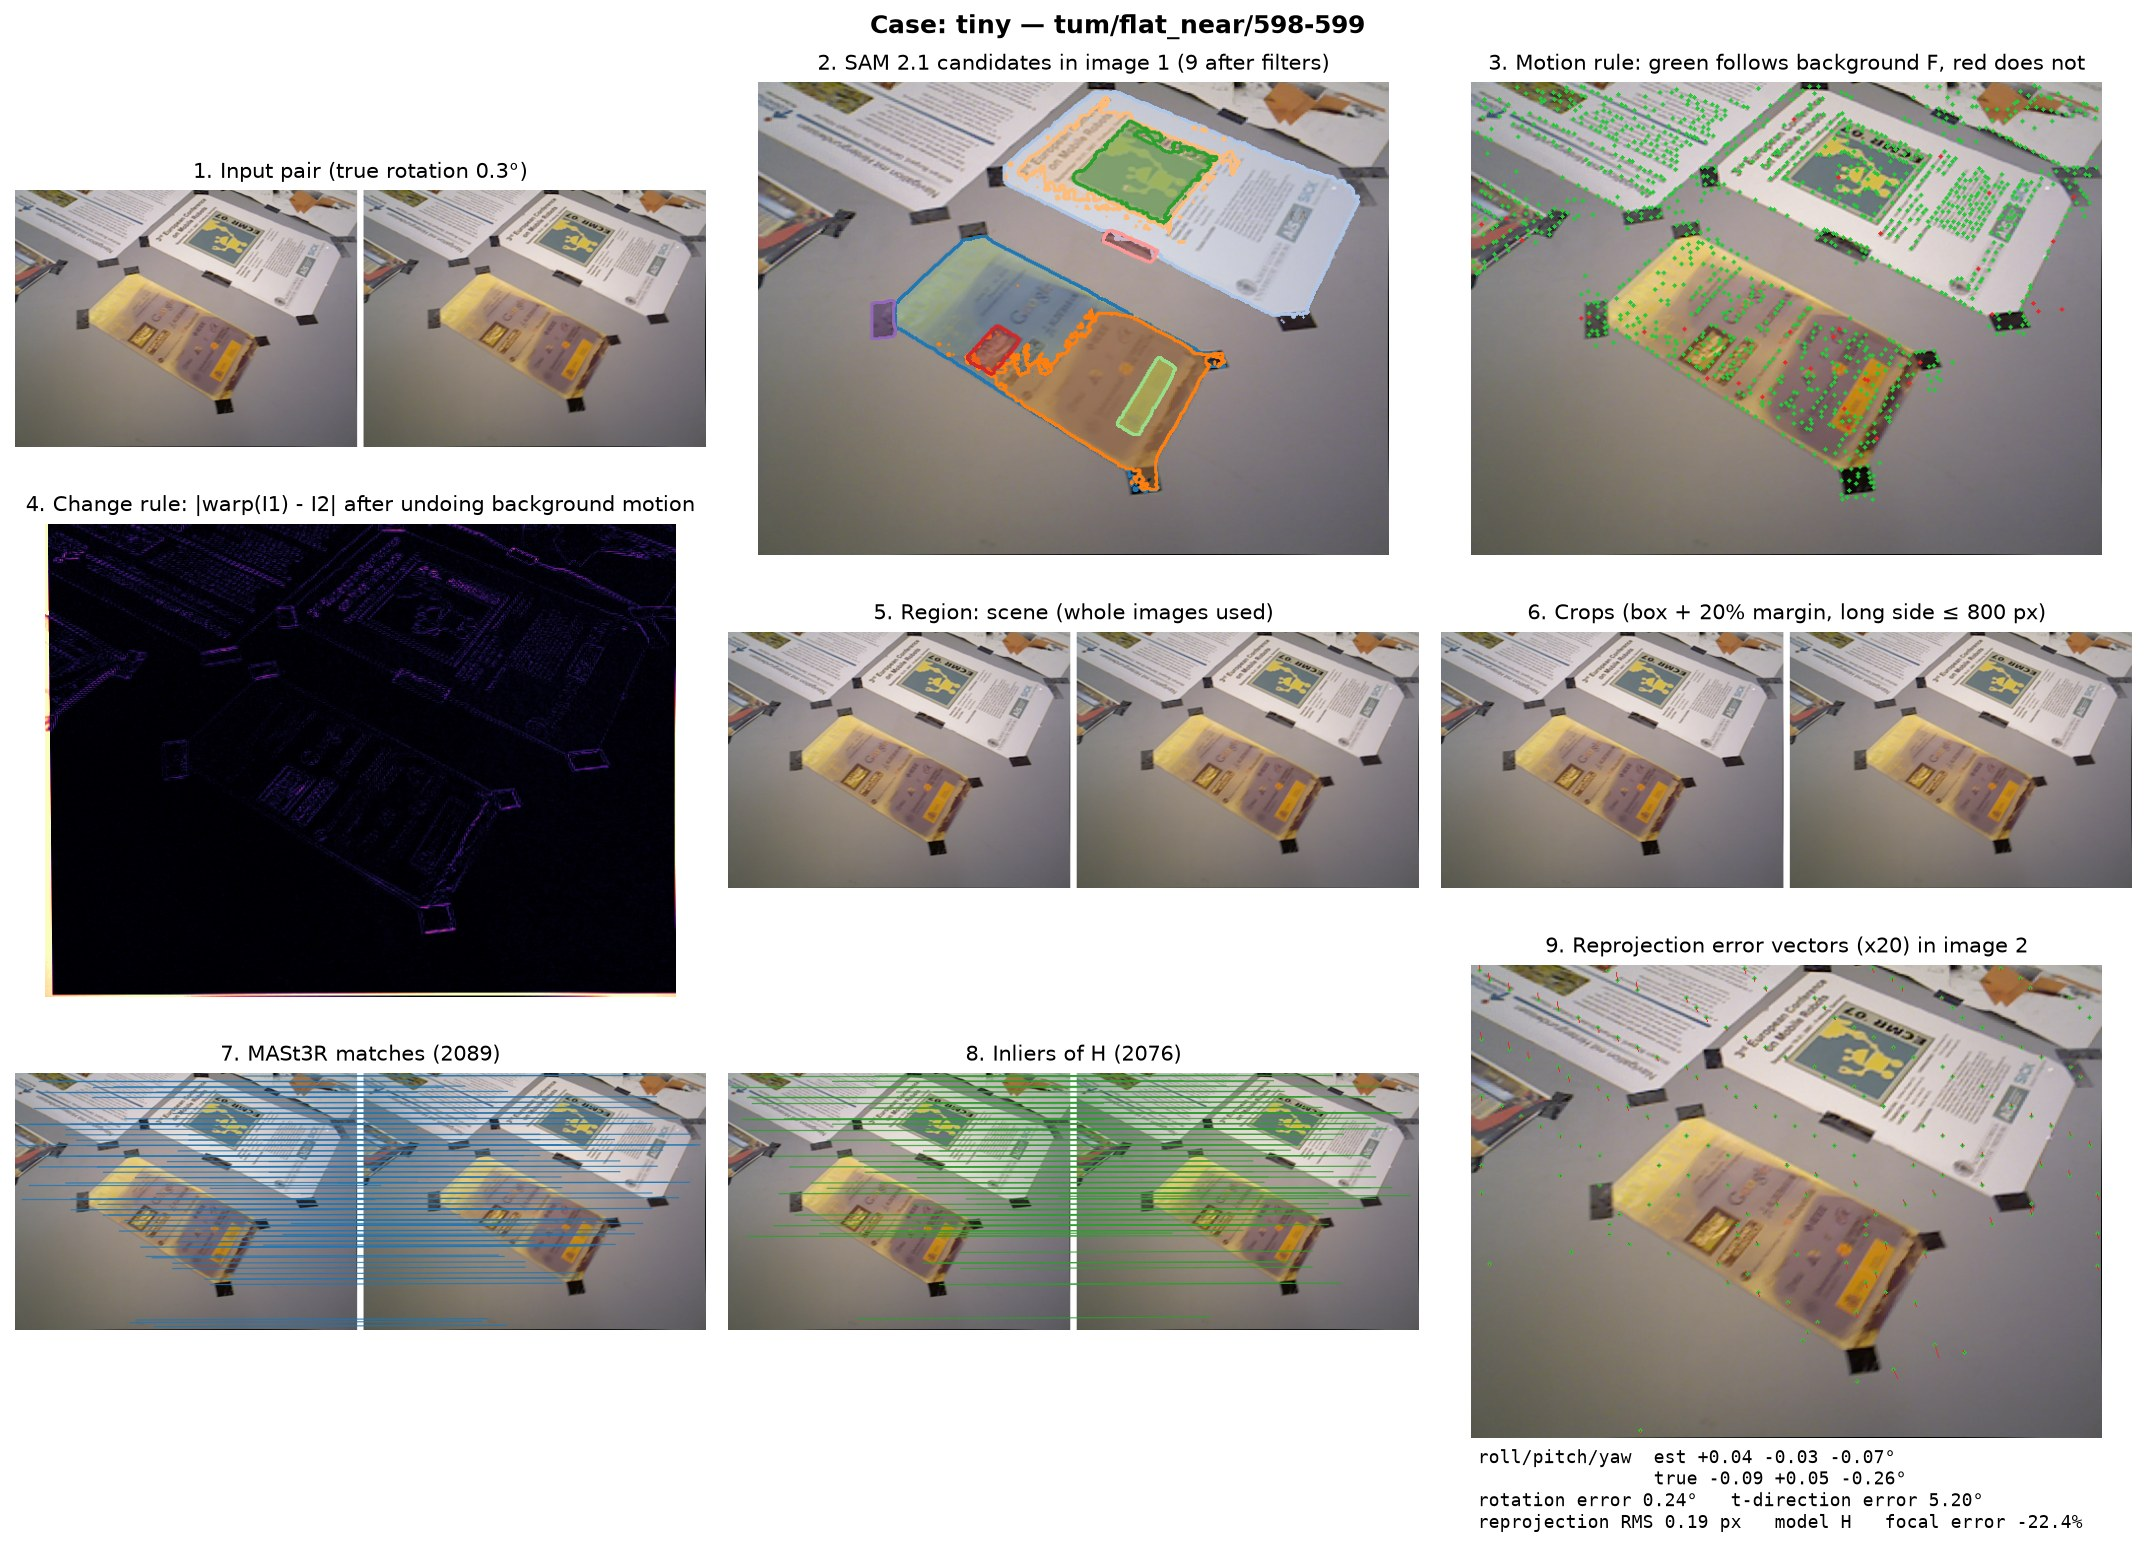
\includegraphics[width=\textwidth]{case_tiny.jpg}
  \caption{Consecutive frames (TUM poster): rotation error $0.24^\circ$; the translation direction is not observable at this baseline.}
  \label{fig:case-tiny}
\end{figure*}

\subsection{Component Study with Known Intrinsics and Regions}
On 751 test pairs (TUM 142, Objectron 189, CO3D 210, MVImgNet 210) with the dataset intrinsics and object masks, the matchers compare as in Table~\ref{tab:bench}.

\begin{table}[H]
\centering\small\setlength{\tabcolsep}{3pt}
\resizebox{\columnwidth}{!}{%
\begin{tabular}{lcccccc}
\toprule
Method & TUM & Objectron & CO3D & MVImgNet & Mean & s/pair\\
\midrule
SIFT & 65.8 & 50.7 & 18.1 & 8.5 & 35.8 & 0.1\\
XFeat+LightGlue & 67.2 & 58.2 & 32.0 & 28.3 & 46.4 & 0.5\\
LoFTR & 67.1 & 65.2 & 33.1 & 24.4 & 47.5 & 5.4\\
MASt3R & \textbf{76.8} & \textbf{81.5} & \textbf{67.8} & \textbf{65.9} & \textbf{73.0} & 20.2\\
\midrule
\texttt{accurate} & 68.1 & 63.0 & 38.6 & 30.2 & 50.0 & 0.9\\
\texttt{confident} & 70.5 & 77.2 & 57.4 & 51.1 & 64.0 & 0.8\\
\bottomrule
\end{tabular}}
\caption{AUC@10 with dataset intrinsics and object masks (751 test pairs); median seconds per pair on a CPU.}
\label{tab:bench}
\end{table}

\begin{table}[H]
\centering\small
\begin{tabular}{lc}
\toprule
Model & AUC@10\\
\midrule
Homography only & 29.9\\
Essential matrix only & 44.3\\
GRIC per pair & \textbf{44.9}\\
\bottomrule
\end{tabular}
\caption{Model selection with fixed correspondences (ALIKED+LightGlue); GRIC selected the homography on 17\% of pairs. The planar-twin check raised every matcher's mean AUC@10 by 1--3 points.}
\label{tab:gric}
\end{table}

\begin{table}[H]
\centering\small\setlength{\tabcolsep}{4pt}
\begin{tabular}{lcccc}
\toprule
Method & 5--15$^\circ$ & 15--30$^\circ$ & 30--60$^\circ$\\
\midrule
SIFT & 40.2 & 35.7 & 19.2\\
XFeat+LightGlue & 47.1 & 52.6 & 30.3\\
LoFTR & 53.4 & 52.3 & 26.1\\
MASt3R & \textbf{68.3} & \textbf{76.5} & \textbf{72.4}\\
\bottomrule
\end{tabular}
\caption{AUC@10 by viewpoint change with known intrinsics and masks.}
\label{tab:bench-views}
\end{table}

\textbf{Sensitivity to the intrinsics.} With the correspondences fixed and the intrinsic matrix perturbed, a focal-length error of $\pm2\%$ costs about one point of mean AUC@10, $\pm5\%$ about two and $\pm10\%$ about six (Figure~\ref{fig:focal}); shifting the principal point by 5\% of the image size costs 7.6 points. Calibration by Zhang's method~\cite{zhang} on the TUM checkerboard sequence gives a focal length within 2.3\% of the published value.

\begin{figure}[H]
  \centering
  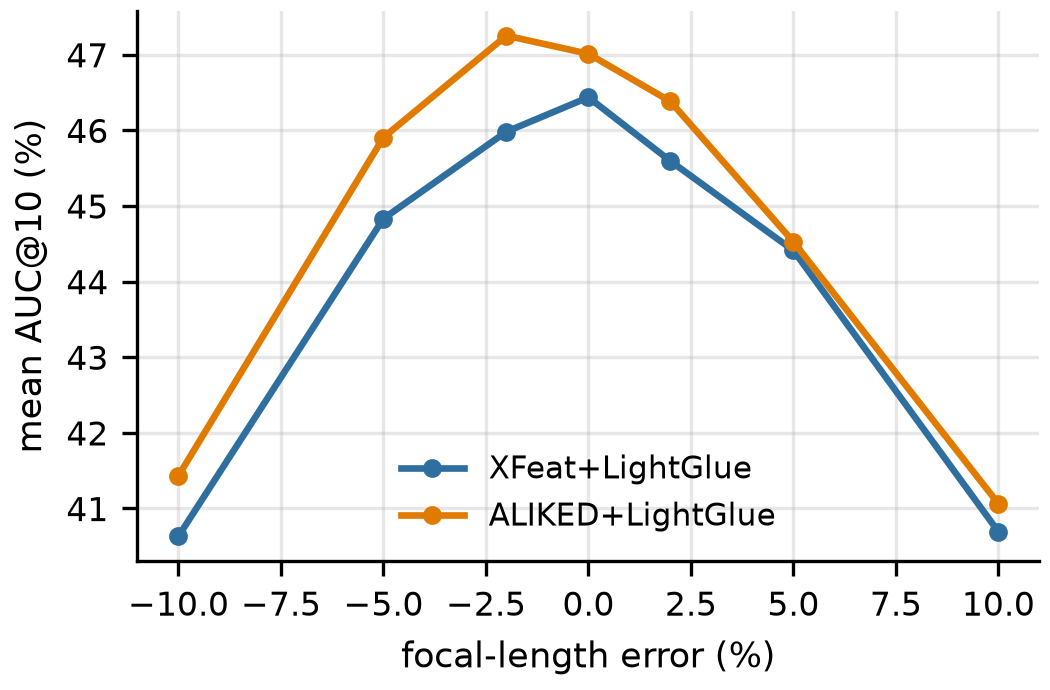
\includegraphics[width=0.9\columnwidth]{focal_sens.png}
  \caption{AUC@10 against the relative error of the focal length.}
  \label{fig:focal}
\end{figure}

\textbf{Object region versus whole image.} With known intrinsics, matching the whole image rather than the object raises AUC@10 on the object datasets (for example 57.8 to 77.1 on Objectron with ALIKED+LightGlue), because in these datasets the object is static and the background carries the same motion; for an object moved independently this would not hold.

\textbf{Verification of the ground truth.} For each dataset, SIFT correspondences on sample pairs lie at a median of 0.2--3.6\,px from the epipolar lines predicted by the converted ground truth on 25 of 28 pairs, against 10--970\,px when the rotation is deliberately transposed (Figure~\ref{fig:checks}).

\begin{figure*}[t]
  \centering
  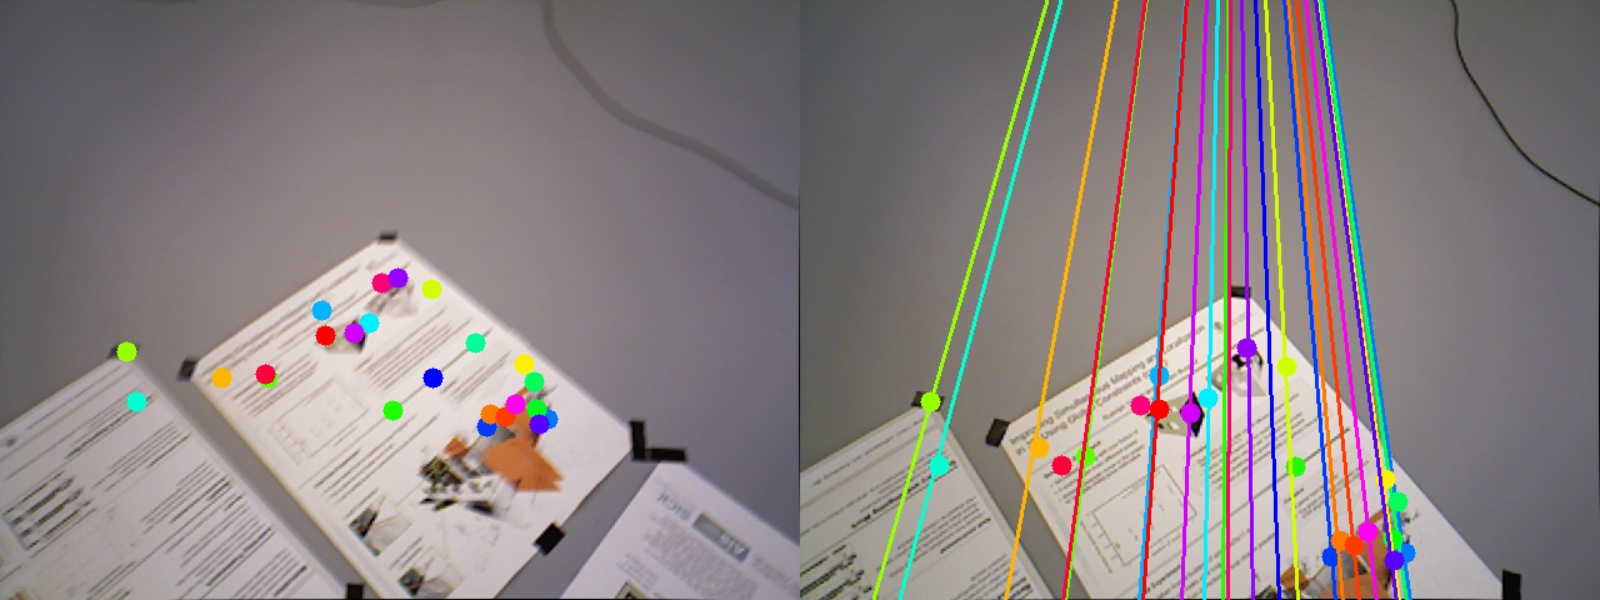
\includegraphics[width=0.32\textwidth]{tum_check.jpg}\hfill
  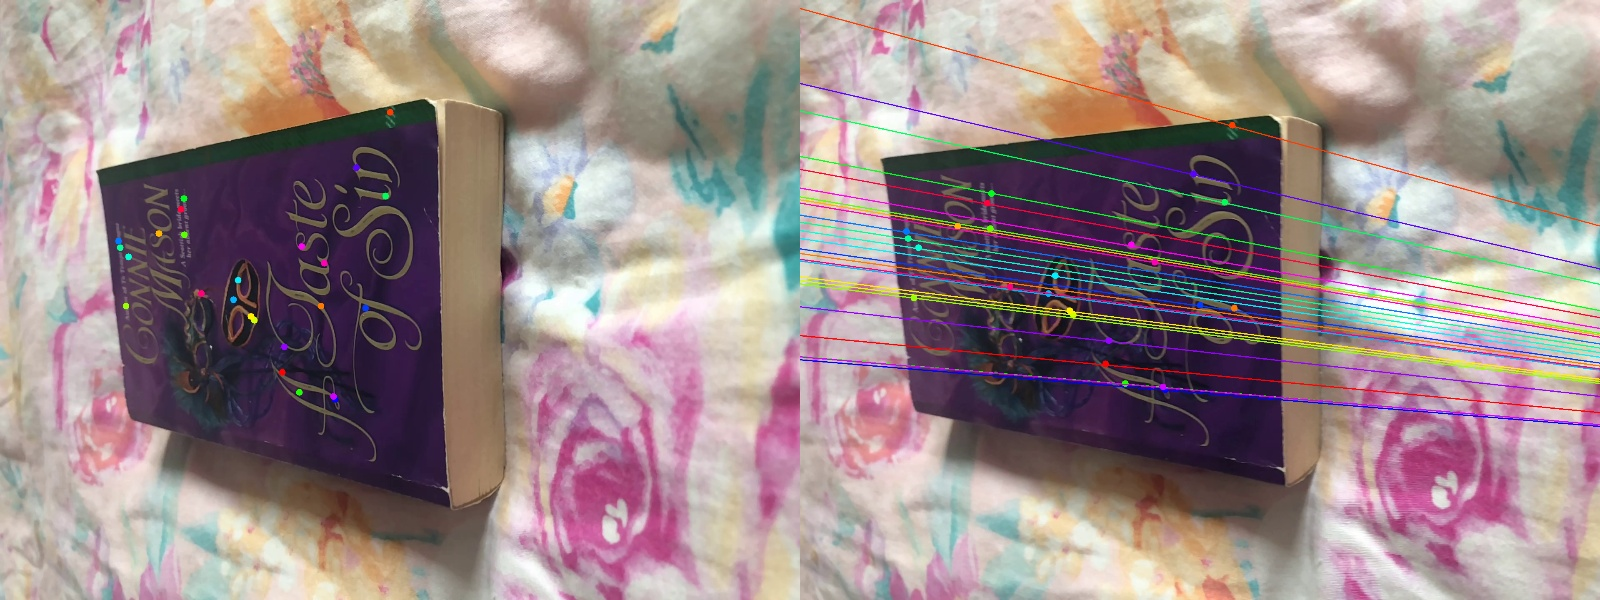
\includegraphics[width=0.32\textwidth]{objectron_check.jpg}\hfill
  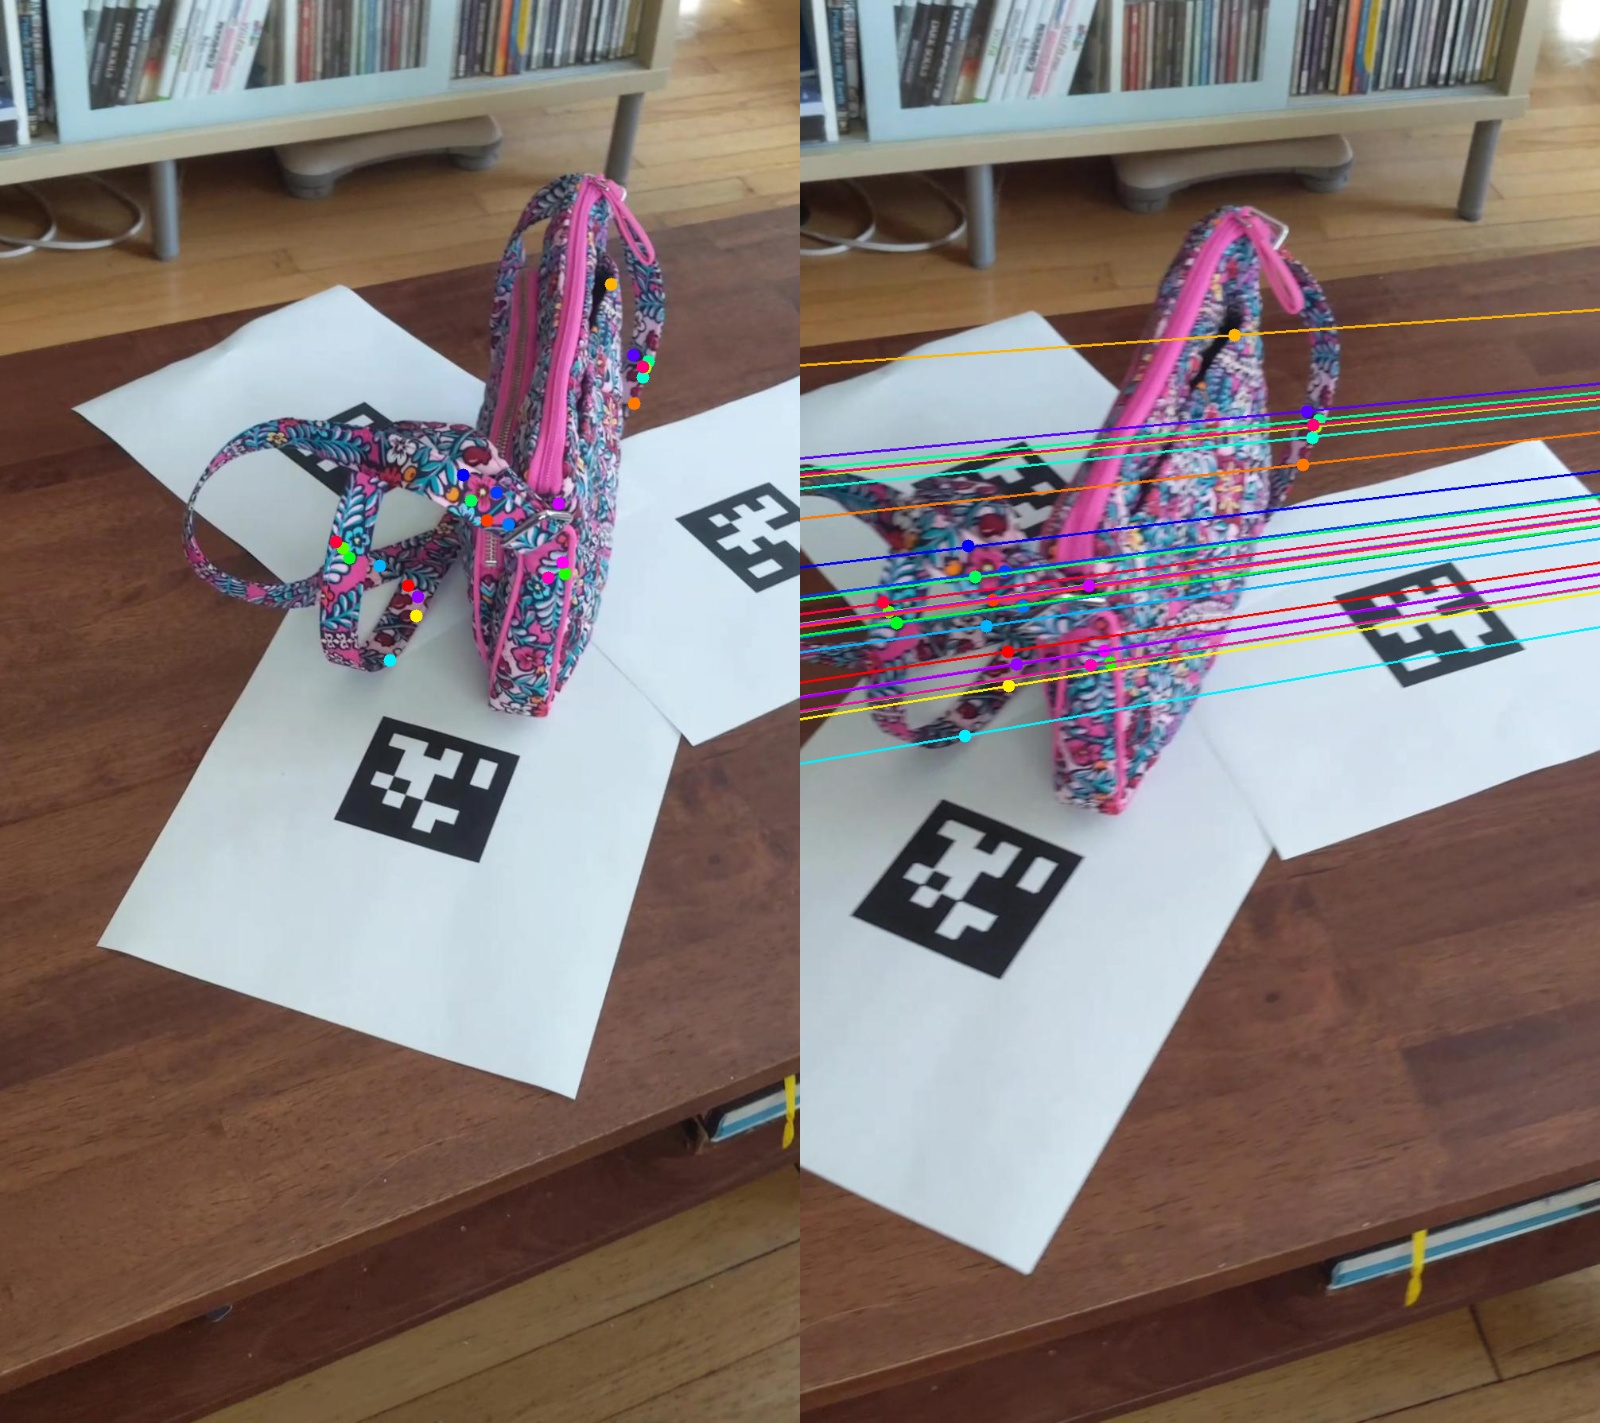
\includegraphics[width=0.32\textwidth]{co3d_check.jpg}
  \caption{Epipolar verification of the ground-truth conversion for TUM, Objectron and CO3D.}
  \label{fig:checks}
\end{figure*}

\begin{figure}[H]
  \centering
  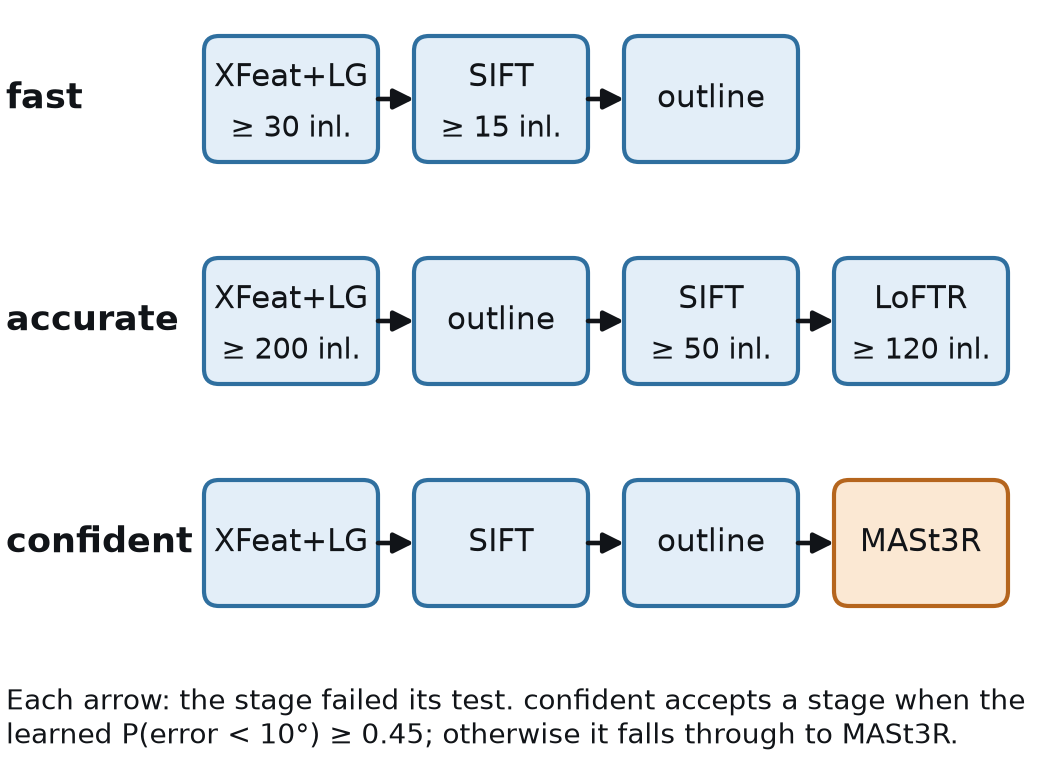
\includegraphics[width=\columnwidth]{cascades.png}
  \caption{Stages of the \texttt{fast}, \texttt{accurate} and \texttt{confident} presets.}
  \label{fig:cascades}
\end{figure}

\end{document}
